\documentclass[a4paper]{article} 
\usepackage[longend,ruled,linesnumbered]{algorithm2e}
\addtolength{\hoffset}{-2.25cm}
\addtolength{\textwidth}{4.5cm}
\addtolength{\voffset}{-3.25cm}
\addtolength{\textheight}{5cm}
\setlength{\parskip}{0pt}
\setlength{\parindent}{0in}

%----------------------------------------------------------------------------------------
%	PACKAGES AND OTHER DOCUMENT CONFIGURATIONS
%----------------------------------------------------------------------------------------

\usepackage{blindtext} % Package to generate dummy text
\usepackage{charter} % Use the Charter font
\usepackage[utf8]{inputenc} % Use UTF-8 encoding
\usepackage{microtype} % Slightly tweak font spacing for aesthetics
\usepackage[italian]{babel} % Language hyphenation and typographical rules
\usepackage{amsthm, amsmath, amssymb} % Mathematical typesetting
\usepackage{float} % Improved interface for floating objects
\usepackage[final, colorlinks = true, 
            linkcolor = black, 
            citecolor = black]{hyperref} % For hyperlinks in the PDF
\usepackage{graphicx, multicol} % Enhanced support for graphics
\usepackage{xcolor} % Driver-independent color extensions
\usepackage{marvosym, wasysym} % More symbols
\usepackage{rotating} % Rotation tools
\usepackage{censor} % Facilities for controlling restricted text
\usepackage{listings, style/lstlisting} % Environment for non-formatted code, !uses style file!
\usepackage{pseudocode} % Environment for specifying algorithms in a natural way
\usepackage{style/avm} % Environment for f-structures, !uses style file!
\usepackage{booktabs} % Enhances quality of tables
\usepackage{tikz-qtree} % Easy tree drawing tool
\tikzset{every tree node/.style={align=center,anchor=north},
         level distance=2cm} % Configuration for q-trees
\usepackage{style/btree} % Configuration for b-trees and b+-trees, !uses style file!
\usepackage[backend=biber,style=numeric,
            sorting=nyt]{biblatex} % Complete reimplementation of bibliographic facilities
\addbibresource{ecl.bib}
\usepackage{csquotes} % Context sensitive quotation facilities
\usepackage[yyyymmdd]{datetime} % Uses YEAR-MONTH-DAY format for dates
\renewcommand{\dateseparator}{-} % Sets dateseparator to '-'
\usepackage{fancyhdr} % Headers and footers
\pagestyle{fancy} % All pages have headers and footers
\fancyhead{}\renewcommand{\headrulewidth}{0pt} % Blank out the default header
\fancyfoot[L]{} % Custom footer text
\fancyfoot[C]{} % Custom footer text
\fancyfoot[R]{\thepage} % Custom footer text
\newcommand{\note}[1]{\marginpar{\scriptsize \textcolor{red}{#1}}} % Enables comments in red on margin



\usepackage{amsmath}
\usepackage{amsfonts}
\usepackage{tcolorbox}
%----------------------------------------------------------------------------------------

\usepackage{listings}
\usepackage{color}
\usepackage{minted}
\usemintedstyle{vs}
\definecolor{dkgreen}{rgb}{0,0.6,0}
\definecolor{gray}{rgb}{0.5,0.5,0.5}
\definecolor{mauve}{rgb}{0.58,0,0.82}

\lstset{frame=tb,
  language=Java,
  aboveskip=3mm,
  belowskip=3mm,
  showstringspaces=false,
  columns=flexible,
  basicstyle={\small\ttfamily},
  numbers=none,
  numberstyle=\tiny\color{gray},
  keywordstyle=\color{blue},
  commentstyle=\color{dkgreen},
  stringstyle=\color{mauve},
  breaklines=true,
  breakatwhitespace=true,
  tabsize=3
}

\begin{document}

%-------------------------------
%	TITLE SECTION
%-------------------------------

\fancyhead[C]{}
\hrule \medskip % Upper rule
\begin{minipage}{0.295\textwidth} 
\raggedright
\footnotesize
Andrei Gabriel Taraboi \hfill\\   
\hfill\\
\end{minipage}
\begin{minipage}{0.4\textwidth} 
\centering 
\large 
Processo e Sviluppo del Software\\ 
\normalsize 
\end{minipage}
\begin{minipage}{0.295\textwidth} 
\raggedleft
\hfill\\
\end{minipage}
\medskip\hrule 
\bigskip

%-------------------------------
%	CONTENTS
%-------------------------------
\tableofcontents
\newpage 

\section{Risk analysis}

La gestione dei rischi è quella disciplina che ha come obbiettivo l'identificazione, gestione e eliminazione dei rischi prima che quest'ultimi diventino una minaccia per il progetto. 

Che cos'è un rischio? Definiamo \textbf{rischio} come la possibilità che ci sia un danno. Bisogna cercare di prevenire un evento che può portare ad un danno serio. 

Definiamo \textbf{risk exposure}(RE), che è una grandezza (calcolabile), per calcolare quanto un progetto sia esposto ad un rischio. Viene calcolato come: 
$RE = P(UO) \cdot L(UO)$. Dove \begin{itemize}
    \item \textbf{P(UO)} è la probabilità di un \textit{unsatisfactory outcome}, ovvero la probabilità che effettivamente un danno (o comunque un risultato non soddisfacente) sia prodotto.
    \item \textbf{L(UO)} è l'entità del danno stesso, ovvero è la perdita per le parti interessate se il risultato non è soddisfacente.
    \end{itemize}
    
Definiamo \textbf{outcome unsatisfactory (\textit{risultato non soddisfacente})} come un risultato non positivo che riguarda diverse aree:
\begin{itemize}
    \item \textbf{utenti} come un progetto che presenta le funzionalità sbagliate, una UI carente, problemi di prestazioni o di affidabilità etc$\ldots$. In questo caso se i problemi sono gravi si hanno alti rischi, come l'utenza che smette di usare il prodotto, portando al fallimento del prodotto, o anche a conseguenze legali.
    \item \textbf{Per gli sviluppatori} con rischi che per esempio si ritrovano superamento del budget e prolungamenti delle scadenze impostate
    \item \textbf{Manutentori}, si possono ritrovare con dei componenti di qualità bassa software e/o hardware
\end{itemize}

Se abbiamo un rischio che produce un \textit{outcome unsatisfactory} il primo elemento su cui soffermarsi è lo studio degli eventi che abilitano il rischio, detti \textbf{risk triggers}. Questo perché per prevenire un rischio, quello che possiamo fare è andare a lavorare sui suoi trigger, fare così in modo che questo rischio non sia mai abilitato. I trigger non sempre sono facili da trovare. 

Quando parliamo dei rischi da un punto di vista della classificazione è utile distinguerne due classi principali di rischio.
\begin{enumerate}
    \item Quelli relativi al processo: Abbiamo dei problemi nel processo di sviluppo software (costi, risorse, tempi)
    \item Quelli relativi al prodotto: Ha a che vedere con il prodotto software, in questo caso possiamo pensare ai fallimenti riguardanti la qualità del prodotto (sicurezza, prestazioni etc$\ldots$) o la distribuzione dello stesso
\end{enumerate} 
    \textbf{Entrambe le classi possono portare al fallimento del progetto e quindi
  vanno gestite entrambe.}
  
Cosa possiamo fare per gestire i rischi? Ci sono due fasi per la gestione dei rischi:
\begin{enumerate}
    \item Risk assessment:  si lavora per identificare quelli che sono i rischi più importanti/rilevanti che devono essere controllati. In questa fase si hanno:
    \begin{itemize}
        \item \textbf{Risk identification} Identificazione dei principali rischi
        \item \textbf{Risk Analysis} analisi dei rischi identificati (tramite calcolo del \textit{risk exposure} e studio dei triggers).
        \item \textbf{Risk prioritization}, che consiste nella prioritizzazione dei rischi analizzati, per focalizzarsi sui più pericolosi per poi scalare ai meno pericolosi.
    \end{itemize} Alla fine, dalla fase di prioritizzazione, si produce una lista dei rischi. LA stessa lista entra nella parte di \textbf{Risk control}.
    \item Risk control e consiste, in primis, sul \textbf{risk management planning}, producendo piani di controllo di due tipi:
    \begin{enumerate}
        \item Di managment: gestione del rischio prima che il rischio si verifichi 
        \item Di contingency: cosa fare quando il rischio si verificherà. Questo succede qualora il \textit{piano di management} fallisca, ci serve quindi sapendo cosa fare a priori in caso di emergenza.
    \end{enumerate} si hanno anche due sotto-fasi per i due tipi di piani:\textbf{risk monitoring} e \textbf{risk resolution}.\\
    Le due fasi vengono ciclicamente ripetute perché i rischi, con il progredire dello sviluppo, variano.  
\end{enumerate}

\subsection{Risk identification}
Come facciamo a identificare i rischi che possono colpire un progetto? Una procedura complessa. 
Un modo per farlo potrebbe essere l'utilizzo di una \textbf{check-list}, includono un insieme di rischi molto comuni a molti progetti. L'analista scorre tale lista cercando rischi che possono essere applicati al progetto in analisi.

Alcuni rischi, in astratto, possono verificarsi sempre ma, il rischio che si sta considerando, va preso in considerazione solo per \textbf{ motivi specifici identificabili} nel mio progetto.\\
Alcune alternative alla \textbf{check-list}, possono essere le riunioni di confronto, \textit{brainstorming}, \textit{workshop} oppure il confronto con prodotti/organizzazioni correlate (confronto con prodotti simili). 

\subsection{Risk analysis}
Per analizzare i rischi si sfrutta esperienza delle reali probabilità che un rischio diventi realtà. Anche in questo si hanno degli schemi su cui basarsi: come \textit{modelli di stima dei costi}, \textit{modelli delle prestazioni}, etc$\ldots$ basati su \textit{simulazioni}, \textit{prototipi}, \textit{analogie con altri progetti} e \textit{check-list} (con stime di probabilità e danno).\\ Le stime sono molto specifici sul singolo progetto.

La parte dell'analisi dei rischi può anche implicare una analisi volta a prendere delle decisioni ai fini di minimizzare il risk exposure, scegliendo o meno tra varie opzioni, scegliendo in modo guidato dai rischi. Per farlo, possiamo utilizzare il decision tree, dove la radice dell'albero che rappresenta il problema. Successivamente andiamo a verificare i vari scenari e successivamente, per ogni scenario, andiamo a calcolare la probabilità che quel scenario si verifichi e poi andiamo a stimare il danno che quel scenario può causare. 

%\begin{figure}[H]
%  \centering
%  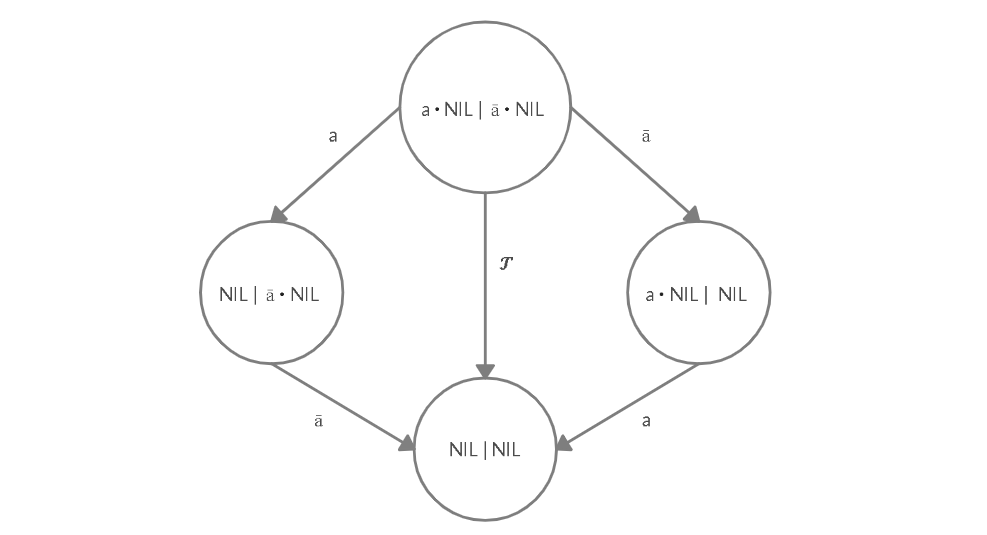
\includegraphics[scale = 0.2]{immagini/Cattura.PNG}
%  \caption{Esempio di decision tree}
%  \label{tree}
%\end{figure}

Si hanno di volta in volta i vari scenari, con le stime di probabilità di trovare un errore critico, di fallimento, di non trovare errori critici etc$\ldots$. Tali probabilità verranno usate per il calcolo del \textit{risk exposure} insieme ad un quantificatore di $L(UO)$ spesso pari all'effettivo costo che conseguirebbe al risultato ottenuto. Infine i vari \textit{risk exposure} di ogni caso vengono sommati per ottenere il \textit{risk exposure} finale.

Ragionando sulle cause dei rischi, andiamo ad analizzare il \textbf{Risk tree} (è uno strumento). Alla radice del \textbf{risk tree} abbiamo il rischio. Trovioamo successivamente una serie di nodi, ogni nodo rappresenta un evento/condizione che a sua volte può essere scomposto in eventi/condizioni fino ad arrivare ad eventi \textbf{foglia}. La scomposizione è guidata da due tipologie di nodi logici:
\begin{enumerate}
    \item \textbf{AND-node}: dove i figli di tali nodi sono eventi legati da una condizione logica \textit{and} (i nodi figlio devono tutti verificarsi affinché il nodo padre si verifichi come conseguenza): dove i figli di tali nodi sono eventi legati dal un \textit{or} (basta che si verifichi uno dei figli)
    \item \textbf{OR-node}
\end{enumerate}

Dato un \textit{risk tree} cerco le combinazioni di eventi atomici che possono portare al rischio, questo perché quello che noi vogliamo è lavorare su queste combinazione per fare si che non si verifichino. Per farlo si esegue una operazione di \textbf{cut-set tree derivation} ovvero, partendo dalla radice scendendo verso le foglie, si riporta in ogni nodo la combinazione (o le combinazioni) di eventi che possono produrre il fallimento. A questo punto si vanno a calcolare le varie combinazioni degli eventi foglia. Praticamente si deriva un insieme di eventi non scomponibili sulle combinazioni dell'\textit{and}.

\subsection{Risk Prioritization}
Bisogna innanzitutto capire da quali rischi partire. Per farlo si pongono(mappano) i valori di $P(UO)$ e $L(UO)$ in un range, per esempio, da 1 a 10, ricalcolando il \textit{risk exposure}. Una volta fatto si lavora in base al \textit{risk-exposure} (che può anche essere un intervallo se le probabilità o i costi sono in un certo intervallo). Una volta effettuato il mapping dei valori ed è stato calcolato il necessario, possiamo eseguire un plotting portando sull'asse y la probabilità di verificarsi di un rischio (\textbf{P(UO)}, sull'asse x l'entità del danno (\textbf{L(UO)}) e poi ogni stima (RE), se precisa diventa un puntino, altrimenti viene rappresentato come un segmento all'interno del plot.  \\
I dati rappresentati mi permettono di segnare delle curve, quest'ultime rappresentano l'entità dei rischi più pericolosi. 

\subsection{Risk Control}
Avendo capito come sono stati prioritizzazti bisogna capire come gestirli.
Per ogni rischio si va a sviluppare un piano di gestione di quest'ultimo, questo piano diventa un vero e proprio documento composto dalle seguenti sezioni:
\begin{itemize}
    \item cosa si sta gestendo 
    \item come mitigare il rischio e quando farlo
    \item di chi è la responsabilità
    \item come approcciarsi al rischio
    \item il costo dell'approccio al rischio
\end{itemize}
Ma cosa facciamo per gestirli? Anche in questo caso vengono utilizzate le check-list che contengono l'insieme di tecniche di risk-managment più comuni in base al rischio specifico. 

Ci sono però alcuni aspetti più generali da considerare:
    \begin{itemize}
      \item \textbf{Reduce risk likehood}: lavorare sulla probabilità che il rischio avvenga, sulla probabilità dei  triggers. Bisogna capire come diminuire la probabilità.
      \item \textbf{Avoid risk}: lavorare, nel limite del possibile, sull'eliminazione stessa del rischio.
      \item \textbf{Reduce consequence likehood}: lavorare sulla riduzione della probabilità di avere conseguenze al danno, non viene quindi ridotto il rischio, ma vengono ridotte le probabilità del danno.
      \item \textbf{Avoid risk consequence} lavorare, nel limite del possibile, sull'eliminazione stessa del danno conseguente al rischio.
      \item \textbf{Mitigate risk consequence} lavorare sul mitigare le conseguenze di un rischio, diminuendo l'entità
      del danno.
    \end{itemize}
    
Bisogna anche studiare le contromisure, da scegliere e attivare in base alla situazione. Si hanno due metodi quantitativi principali per ragionare quantitativamente sulle contromisure:
\begin{itemize}
    \item \textbf{Risk-Reduction Leverage}, si calcola quanto una certa contromisura può ridurre un certo rischio  secondo la seguente formula: $\displaystyle RRL(r, cm)=\frac{RE(r)-RE(\frac{r}{cm})}{Cost(cm)}$ \\
    Dove $r$ rappresenta il rischio, $cm$ la contromisura e $\frac{r}{cm}$ la contromisura $cm$ applicata al rischio $r$. Calcolo quindi la differenza tra \textit{risk exposure} del rischio $r$ e quella avendo considerando la contromisura $cm$. Divido il risultato per il costo della contromisura.\\ La miglior contromisura è quella con il RRL maggiore, avendo minor costo e maggior efficacia dal punto di vista del \textit{risk exposure}.
    \item \textbf{Defect Detection Prevention, DDP}
    Questo metodo confronta le varie contromisure, confrontando anche gli obiettivi del progetto, in modo quantitativo e fa un confronto indiretto producendo matrici in cui si ragiona in modo indipendente sulle singole contromisure e sui singoli rischi ma il risultato finale è un confronto tra tanti rischi e tante misure che possiamo prendere in considerazione contemporaneamente. Si ha un ciclo di 3 passaggi:
    \begin{enumerate}
        \item Elaborare la matrice di impatto dei rischi. Questa matrice calcola l'impatto dei rischi sugli obiettivi principali (presi in considerazione) del progetto. 
        I valori della matrice, ovvero $impact(r, obj)$ (che ha per colonne i rischi $r$ e righe gli obiettivi del progetto $obj$) variano da 0, nessun impatto, a 1, completa perdita di soddisfazione (e totale non raggiungimento dell'obiettivo indicato). Ogni rischio viene accompagnato dalla probabilità $P$ (likehood) che accada. Ogni obiettivo è accompagnato dal \textbf{peso} $W$ che ha nel progetto (la somma di tutti i pesi è pari a 1). 
        
        Si possono calcolare altri valori di sintesi. In primis la \textbf{criticità} di un rischio rispetto a tutti gli obiettivi indicati: \[criticality(r)=P(r)\cdot\sum_{obj}(impact(r, obj)\cdot W(obj))\] La criticità sale se sale l'impatto e se sale la probabilità del rischio.\\ Un altro dato è la \textbf{perdita di raggiungimento} di un obiettivo qualora tutti i rischi si verificassero: \[loss(obj)=W(obj)\cdot\sum_{r}(impact(r, obj)\cdot P(r))\]
        
        \item elaborare contromisure efficaci per la matrice elaborata. In questa fase si usa il fattore di criticità del rischio. Viene prodotta una nuova matrice con colonne pari ai rischi (con probabilità e criticità) e righe pari alle contromisure. I valori presenti nelle celle saranno le riduzioni di rischio di una contromisura $cm$ sul rischio $r$ ($reduction(cm,r)$). La riduzione va da 0, nessuna riduzione, a 1, rischio eliminato. \\
        Si possono calcolare altri valori di sintesi. Possiamo calcolare la \textbf{combineReduction}, che ci dice quanto un rischio viene ridotto se tutte le contromisure che abbiamo identificato sono attivate: \[combineReduction(r)=1-\prod_{cm}(1-reduction(cm, r))\] 
        
        Un altro valore è l'\textbf{overallEffect}, ovvero l'effetto di ogni contromisura sull'insieme dei rischi considerato: \[overalleffect(cm)=\sum_r(reduction(cm,r)\cdot criticality(r))\] si avrà effetto maggior riducendo rischi molto critici \item determinare il bilanciamento migliore tra riduzione dei rischi e costo delle contromisure. Bisogna considerare anche il costo di ogni contromisure e quindi si fa il rapporto tra effetto di ciascuna contromisura e il suo costo e scegliendo il migliore
    \end{enumerate}
\end{itemize}

Analizzando il \textbf{Managment and Contingecy Plan}, dove il managment plan che definisce le azioni per prevenire il rischio, e il contingecy plan che indica quello che dobbiamo fare qualora si verifichi il rischio. 

Si passa quindi al \textbf{risk monitoring/resolution}. Queste due parti sono tra loro integrate. I rischi vanno monitorati e occorrenza vanno risolti il prima possibile. Tutte queste attività sono costose e si lavora su un insieme limitato di rischi, una decina, in base alle risorse disponibili.

\section{CMMI - Capabilty Maturity Model Integration}
Il \textbf{Capability Maturity Model Integration (\textit{CMMI})} è un programma di formazione e valutazione per il miglioramento a livello di processo gestito dal \textit{CMMI Institute}.\\ 
Bisogna prima introdurre il concetto di \textbf{maturità dei processi}. 
La probabilità di portare a termine un progetto dipende dalla \textit{maturità del progetto} e la maturità dipende dal grado di controllo che si ha sulle azioni che si vanno a svolgere per realizzare il progetto. 
Si ha quindi che: 
    \begin{itemize} \item il progetto è \textbf{immaturo} quando le azioni legate allo sviluppo non sono ben definite o ben controllate e quindi gli sviluppatori hanno troppa libertà che rischia di degenerare in una sorta di anarchia nel controllo del processo di sviluppo, alzando la probabilità di fallimento 
    \item il progetto è \textbf{maturo} quando le attività svolte sono ben definite, chiare a tutti i partecipanti e ben controllate. Si ha quindi un modo per osservare quanto si sta svolgendo e verificare che sia come pianificato, alzando le probabilità di successo e riducendo quelle di fallimento.
\end{itemize}

La \textbf{maturità del processo} è definita tramite un insiemi di livelli di maturità con associate metriche per gestire i processi, questo è detto \textbf{Capability Maturity Model (\textit{CMM})}. In altri termini il modello CMM è una collezione dettagliata di \textit{best practices} che aiutano le organizzazioni a migliorare e governare tutti gli aspetti relativi al processo di sviluppo.
%%% foto del diagramma 
\begin{figure}[H]
    \centering
    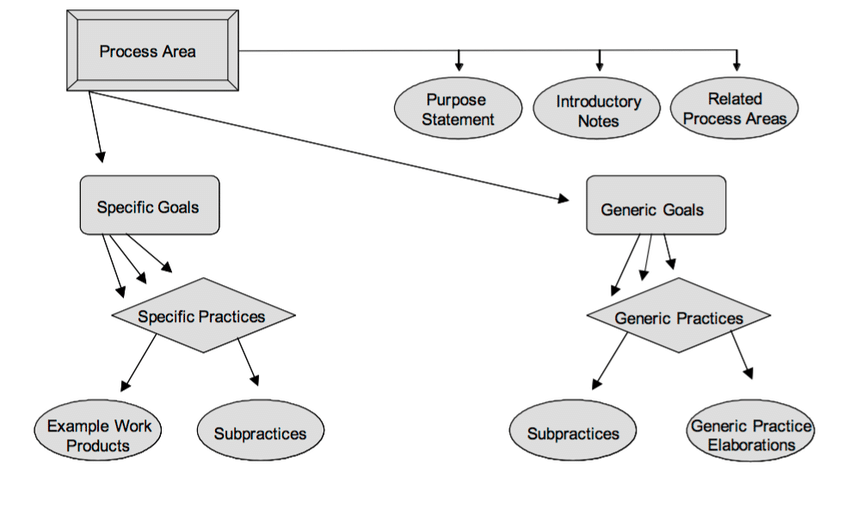
\includegraphics[scale = 0.4]{Imm/CMMI-Dev-Model-components-in-Tea10.png}
    \label{fig:my_label}
\end{figure}
All'interno del diagramma notiamo: 
\begin{itemize} 
    \item \textbf{Process area}, che racchiude al suo interno una collezione di pratiche organizzate secondo obiettivi, e riguarda una certa area del processo di sviluppo software. Nel CMMI abbiamo 22 diverse \textit{process area}, tra cui \textit{configuration management}, \textit{project planning}, \textit{risk management}, $\dots$. Nel diagramma si ha lo studio di una generica \textit{process area}, ciascuna \textbf{process area} ha: 
        \begin{itemize} 
            \item un \textbf{purpose statement}, che descrive lo scopo finale della \textit{process area} stessa 
            \item un \textbf{introductory notes}, con nel note introduttive che descrivano i principali concetti relativi alla \textit{process area} 
            \item un \textbf{related process area}, che contiene la lista delle altre \textit{process area} correlate a quella corrente, se presenti.
        \end{itemize} 
    \item le \textbf{process area} si dividono in due \textit{tipologie di obiettivi}: 
        \begin{enumerate} 
            \item \textbf{specific goals}, ovvero gli obiettivi specifici della singola \textit{process area} in questione. Questi obiettivi caratterizzano la \textit{process area} 
            \item \textbf{generic goals}, ovvero gli obiettivi comuni a \textbf{tutte} le \textbf{process area}. Questi obiettivi rappresentano quanto la \textit{process area} sia ben integrata e definita nel contesto del processo ma questi criteri sono generali 
        \end{enumerate} 
    \item all'interno di ogni \textbf{specific goals} abbiamo una serie di \textbf{specific practices}, ovvero quelle azioni che se svolte permettono di raggiungere quell'obiettivo specifico e, a loro volta, tali pratiche sono organizzate in: 
        \begin{itemize} 
            \item \textbf{example work product}, ovvero elenchi di esempi di prodotti che possono essere generati attraverso l'adempimento delle pratiche 
            \item \textbf{subpractices}, ovvero pratiche di grana più fine
        \end{itemize} 
    \item all'interno di ogni \textbf{generic goals} abbiamo una serie di \textbf{generic practices} comuni a tutti, con le pratiche che devono essere svolte per gestire opportunamente una qualsiasi \textit{process area} e a loro volta tali pratiche sono organizzate in: 
        \begin{itemize} 
            \item \textbf{generic practices elaborations}, ovvero ulteriori informazioni di dettaglio per la singola pratica
            \item \textbf{subpractices}, ovvero pratiche di grana più fine 
        \end{itemize} 
\end{itemize}

Per capire quanto bene un processo software è organizzato secondo questo standard bisogna mappare quali goals e quali pratiche si stanno perseguendo e seguendo e usare CMMI non solo come ispirazione, ma come vero e proprio \textbf{standard} per definire le azioni da svolgere nonché per confrontare il nostro operato e studiarlo qualitativamente. Lo studio qualitativo mi permette di stabilire la \textbf{maturità} del progetti, secondo un certo livello di \textit{compliance}, detto \textbf{CMMI level}. Tale qualità che può essere certificata da enti certificatori appositi.\\

Ci sono due linee di sviluppo, rispetto a questo standard, che bisogna prendere in considerazione:
\begin{enumerate}
    \item \textbf{capability levels (\textit{CL})}, che cattura e rappresenta quanto bene si sta gestendo una particolare \textit{process area} (quindi ciascuna \textit{process area} può raggiungere un diverso CL). Quindi per una singola \textit{process area} mi dice quanto bene sto raggiungendo i \textit{generic goals} (e di conseguenza anche i vari \textit{specific goals}, in quanto quelli generici impongono il controllo e la documentazione di quelli specifici). 
    Il CL ha valore da 0 a 3: 
        \begin{itemize} 
            \item \textbf{level 0: \textit{incomplete}}, dove probabilmente non si stanno nemmeno svolgendo tutte le pratiche richieste per quella \textit{process area} o sono state svolte solo parzialmente 
            \item \textbf{level 1: \textit{performed}}, dove si eseguono le pratiche e i vari \textit{specific goals} sono soddisfatti 
            \item \textbf{level 2: \textit{managed}}, dove oltre alle pratiche si ha anche una gestione delle attività stesse, come indicato nello standard.
            \item \textbf{level 3: \textit{defined}}, dove l'intero processo è ben definito secondo lo standard, descritto rigorosamente e si ha un processo completamente su misura dell'organizzazione 
        \end{itemize} 
    I CL di ciascuna \textit{process area} possono essere rappresentate su un diagramma a barre, dove viene indicato il CL attuale e il \textbf{profile target}, ovvero il livello a cui quella \textit{process area} deve arrivare (che non è per forza il terzo). 
    
    \item \textbf{maturity levels (\textit{ML})}, che cattura il livello raggiunto dall'intero processo di sviluppo ragionando su tutte le \textit{process area} che sono state attivate. Rappresenta quanto bene si sta lavorando sull'insieme intero della \textit{process area}. 
    A livello di grafico punta direttamente all'elemento specificante la \textit{process area}. Il ML ha valore da 1 a 5: 
        \begin{itemize} 
            \item \textbf{level 1: \textit{initial}}, dove si ha un processo gestito in modo caotico, scarso controllo
            \item \textbf{level 2: \textit{managed}}, dove si ha già un processo ben gestito secondo varie policy 
            \item \textbf{level 3: \textit{defined}}, dove si ha un processo ben definito secondo lo standard aziendale 
            \item \textbf{level 4: \textit{quantitatively managed}}, dove si stanno anche raccogliendo dati che misurano quanto bene sta andando bene il processo, facendo quindi una misura quantitativa dello stesso 
            \item \textbf{level 5: \textit{optimizing}}, dove grazie alle informazioni raccolte nel livello precedente ottimizzo il processo, in un'idea di \textit{continuous improvement} del progetto stesso 
        \end{itemize} 
    Gli ultimi due livelli sono davvero difficili da raggiungere.
\end{enumerate}

Tra i principali \textit{generic goals (GG)} abbiamo: 
\begin{itemize} 
    \item \textit{GG1}: raggiungere i \textit{specific goals}, tramite l'esecuzione delle \textit{specific practices} 
    \item \textit{GG2}: ufficializzare un \textit{managed process}, tramite training del personale, pianificazione del processo, controllo dei \textit{work product}, $\dots$ 
    \item \textit{GG3}:  ufficializzare un \textit{defined process}, tramite la definizione rigorosa del progetto e la raccolta di esperienze legate al processo 
\end{itemize}
\section{Requirements Engineering}
Ha come obiettivo la comprensione di come una soluzione software, che stiamo sviluppando, si deve comportare per risolvere un determinato problema. Bisogna quindi comprendere quale sia il problema da risolvere e in quale contesto si verifica, per poter arrivare così ad una soluzione corretta ed efficace di problemi reali.\\
Ci andiamo quindi a concentrare su due elementi essenziali: il problema e il contesto in cui il problema si verifica. \\

Stiamo usando una analogia per dire che all'interno del mondo possiamo avere un problema che risolviamo attraverso una macchina(computer)
\subsection{The problem world and the machine solution}
Definiamo le componenti della nostra analogia:
\begin{itemize}
    \item il \textbf{mondo}: presenta un problema derivante e prodotto dal mondo reale, che bisogna risolvere con un calcolatore. Il mondo è composto da:
        \begin{itemize}
            \item \textbf{componenti umani}, quindi staff, operatori, organizzazioni $\dots$
            \item \textbf{componenti fisici} che possiao pensare come device, software legacy, madre natura
        \end{itemize}
    \item \textbf{macchina}: bisogna svilupparla per risolvere il problema. Si compone di un software da sviluppare o comprare e implementazioni hardware associate con device di input e output annessi.
\end{itemize} 
RE si occupa proprio di definire gli effetti della macchina sul problema (sul mondo) identificato, e di definire le assunzioni che possiamo fare nel realizzare la macchina e quali sono le proprietà principali del mondo da prendere in considerazione.
RE studia quindi il mondo e la sua interazione con la macchina, senza definire come funziona internamente la macchina.\\
Ci sono alcuni componenti che costituiscono il \textbf{world phenomena} ed alcuni il \textbf{machine phenomena}, alcuni aspetti però sono condivisi tra le due componenti i \textbf{shared phenomena}.

Quando parliamo di RE è bene distinguere due elementi 
\begin{enumerate}
    \item ogni volta che si prende in considerazione un problema, normalmente esiste sempre un \textbf{system-as-is}, ovvero un sistema preesistente che già risolve il problema (anche se magari in modo non efficiente e qualitativamente insufficiente). Si ha quindi sempre un sistema da cui partire.
    \item il \textbf{system-to-be} è il sistema che si andrà a realizzare, in altre parole è il sistema su cui opererà la \textbf{macchina/software}.
\end{enumerate}
Studiare il \textbf{system-as-is} è essenziale per poter lavorare al \textbf{system-to-be}.

RE è un insieme di attività che hanno come obiettivo quello di esplorare, valutare, documentare, consolidare, rivisitare e adattare gli obiettivi, le capacità, le qualità, i vincoli e le assunzione su un software \textup{system-to-be} basate sul problema sorto dal \textbf{system-as-is } e sulle nuove opportunità tecnologiche.
L’output di queste attività è un \textbf{documento di specifica dei requisiti} con tutto ciò che il sistema deve soddisfare. Se l’output non è un singolo documento si ha una collezione di singoli requisiti, che nel metodo agile sono storie/cards e in altri metodi un repository centrale con un db condiviso contenete i vari requisiti. \\

Altre persone hanno cercato di definire differentemente i requisiti, esplicitando che quando si tende a sviluppare un software se i requirements non sono ben definiti, ci possiamo ritrovare differente da quello desiderato. Risulta necessario capire bene il why, what e how:
\begin{enumerate}
  \item \textbf{why}, perché serve un nuovo sistema in base alle nuove condizioni
  \item \textbf{what}, quale feature del sistema soddisferà il contesto in cui ci troviamo
  \item \textbf{who}, come il sistema deve essere costruito 
\end{enumerate}
RE si occupa degli obiettivi del \textbf{mondo}, per funzioni di vincoli sui sistemi software; e i loro collegamento a specifiche precise del come il software dovrebbe comportarsi. 

In un modello simil-cascata di sviluppo software, l'attività di RE è una delle primissime attività svolte (probabilmente la prima dal punto di vista tecnico), subito dopo quelle di definizione del sistema e di business plan. 
Re si occupa di capire qual è il giusto sistema da sviluppare, prima ancora di pensare al design, all’implementazione e all’evoluzione software, che invece si occupano di ottenere il software giusto, sviluppandolo nel modo corretto.

Sbagliare nell’attività di RE può portare ad un ottimo software che risolve i problemi sbagliati (o non tutti i problemi che dovrebbe risolvere). Lavorare sulla parte di RE è quindi molto difficile:
\begin{itemize}
    \item Si deve ragionare su tante versioni del sistema (broad scope): as-is, to-be e to-be-next (quando si vuole essere lungimiranti sul comportamento del sistema, sapendo e prevedendo evoluzioni future).
    \item Si lavora in ambienti ibridi (broad scope): tra umani, leggi, device, policy, leggi fisiche, quindi in un contesto eterogeneo che va compreso a fondo (ignorare degli aspetti può portare al fallimento).
    \item Si hanno diversi aspetti funzionali, qualitativi e di sviluppo (multiple concerns)
    \item Si hanno diversi livelli di astrazione (multiple abstraction levels): con obiettivi strategici a lungo termine di inserimento sul mercato e dettagli operazionali.
    \item Si hanno tanti stakeholders (multiple stakeholders): quindi diverse parti interessate per le quali risolvere problemi e considerare gli interessi (gestendo i potenziali conflitti tra i vari stakeholders).
    \item Si hanno tante attività tecniche legate tra loro (multiple interwined tasks): conflict management, risk management, evaluation of alternatives, prioritization, quality assurance, change anticipation (per capire cosa fare, in che ordine, con che rischi, con che livelli di qualità).
\end{itemize}


\subsection{Lo scope di RE: la dimensione del why, what e who}
\begin{enumerate}
    \item \textbf{dimensione del why}(why a new system?): dove si identificano, analizzano e rifiniscono i requisiti del \textbf{system-to-be} per: affrontare le carenze analizzate del \textbf{system-as-is}, in linea con gli obiettivi di business, sfruttando le opportunità tecnologiche.\\ 
    Si hanno le seguenti difficoltà:
      \begin{itemize}
        \item acquisire conoscenza del dominio 
        \item valutare opzioni alternative (ad esempio modi alternativi per soddisfare lo stesso obiettivo) 
        \item abbinare problemi-opportunità e valutarli in termini di implicazioni, e rischi associati 
        \item gestire obiettivi contrastanti
      \end{itemize}
    \item \textbf{dimensione del what}(what service?), dove si identificano, analizzano e rifiniscono le funzionalità del \textbf{system-to-be} (servizi software e associate procedure manuali) per soddisfare gli obiettivi individuati in base a vincoli di qualità: sicurezza, prestazioni, $\dots$ basati su ipotesi realistiche sull'ambiente.\\
    Si hanno le seguenti difficoltà:
        \begin{itemize}
            \item identificare il giusto set di funzionalità 
            \item specificarle precisamente per essere comprese da tutte le parti 
            \item garantire la tracciabilità $backward$ per gli obiettivi del sistema. (tornare indietro)
        \end{itemize}
    \item \textbf{dimensione del who}(who will be responsible for what?), dove si assegna responsabilità per gli obiettivi, i servizi, i vincoli tra i componenti del \textbf{system-to-be} in base alle loro capacità e agli obiettivi del sistema, uscendo anche dai confini dell'ambiente software.\\
    La difficoltà è valutare opzioni alternative per decidere il giusto grado di automazione 
\end{enumerate}

\subsection{Tipi di requisiti}
Bisogna anche ragionare sui tipi di requisiti su cui si deve lavorare. Una prima differenza si ha nel modo in cui sono scritti i requisiti:
\begin{itemize} 
    \item \textbf{descriptive statements (\textit{dichiarazioni descrittive})}, che indicano dei requisiti non negoziabili, rappresentano dei comportamenti derivanti dalle leggi del mondo su cui lavora la macchina. Si ha quindi zero margine di modifica 
    \item \textbf{prescriptive statements (\textit{dichiarazioni prescrittive})}, che indicano requisiti negoziabili che riguardano comportamenti che un sistema deve avere ma che volendo possono essere modificati. 
\end{itemize}
Si possono avere requisiti non ovvi, o lo sono solo in un contesto specialistico e quindi spesso non a chi lavora sul software (che generalmente non è del settore).

I requisiti possono inoltre differire per gli elementi che prendono in considerazione:
\begin{itemize}
  \item \textbf{system requirements},  riguardano il comportamento dell’ambiente, per capirne il funzionamento (che andrà ad influenzare il software).
  \item \textbf{software requirements}  riguardano il comportamento del software nell’ambiente, studiando i cosiddetti shared phenomena accennati in precedenza.
\end{itemize}
I requisiti non riguardano mai il comportamento interno del software. Ricordando che: 
\begin{itemize}
    \item $sistema = ambiente + software$
    \item $requisiti \; del \; sistema = requisiti \; software + domain \; properties + assunzioni$
\end{itemize}\label{riferimento}
Dove domain properties sono le leggi valide per un certo ambiente, proprietà immutabili e le assunzioni, che chi realizza il software, su come è fatto l’ambiente. Le assunzioni descrivono gli ambienti compatibili con il software. Se troppo restrittive possono portare al fallimento del progetto che riguarderebbe pochissimi casi particolari.\\

In ottica di un ragionamento di interazione tra sistema software e ambiente citiamo il \textbf{modello Parnas95}, della metà degli anni novanta. In modo elementare, il modello schematizza l’interazione software-ambiente in modo da esplicitare i device usati dal software-to-be per interagire con ambiente. 
\begin{figure}[H]
    \centering
    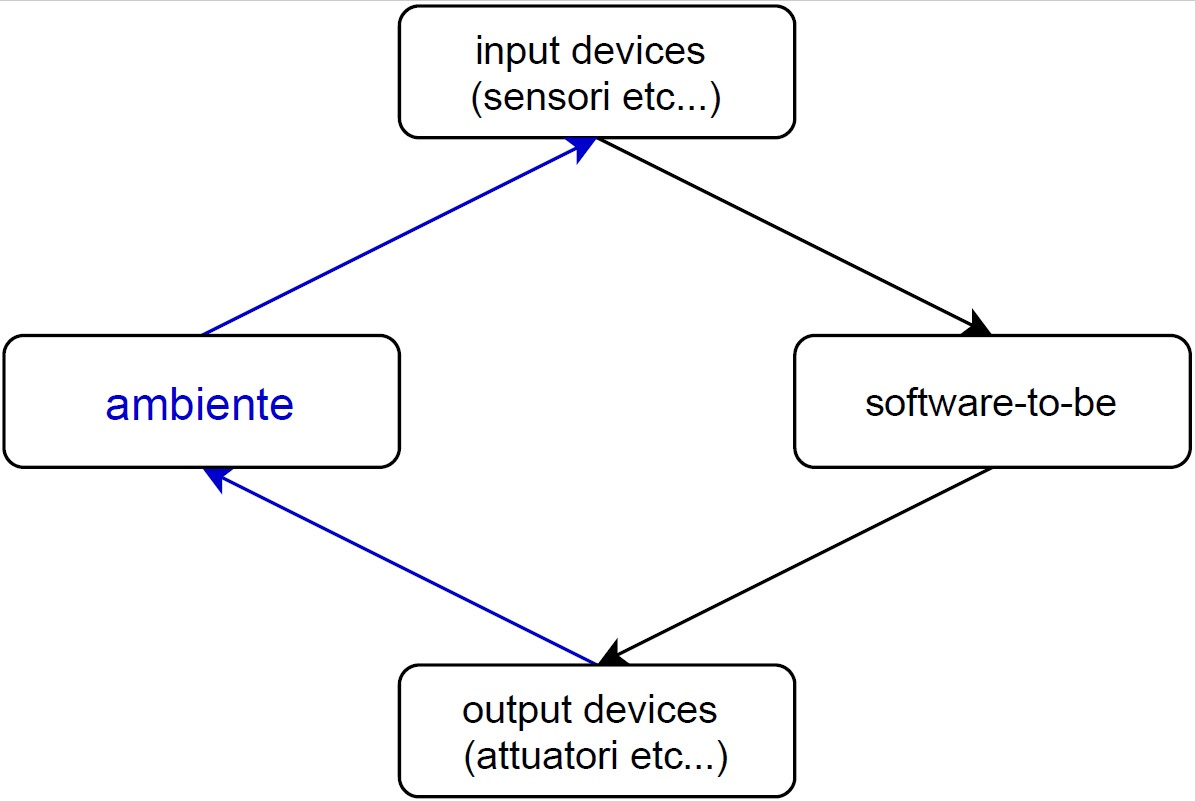
\includegraphics[scale= 0.25]{Imm/re_cose.PNG}
    \caption{Modello Parns95}
    \label{fig:parnas}
\end{figure}
Si ha uno schema composto da:
\begin{itemize}
    \item dei device di input, simil sensori, che percepiscono l’ambiente.
    \item dei device di output che permettono di interagire con l’ambiente.
\end{itemize}
e 4 tipi di variabili:
\begin{enumerate}
  \item \textbf{input data (I)}, tra \textit{input devices} e \textit{software-to-be}
  \item \textbf{output results (O)}, tra \textit{software-to-be} e \textit{output devices}
  \item \textbf{controlled variables  (C)}, tra \textit{output devices} e \textit{ambiente}
  \item \textbf{monitored variables (M)}, tra \textit{ambiente} e \textit{input devices}
\end{enumerate}
E si ha che $\mbox{System requirements}\subseteq M\times C$ e $\mbox{Software requirements}\subseteq I\times O$. Ritornando al comportamento di un software [\ref{riferimento}] avevamo parlato brevemente di dominio e assunzioni. Diremo inoltre che :\\
$\mbox{Assumptions}\subseteq M\times C\cup M\times I \cup C\times O$ \\
Definiamo \textbf{domain property} come un \textit{descriptive statement} sui problemi legati ai fenomeni del \textit{mondo} (a prescindere da qualsiasi \textbf{software-to-be}).\\ Utilizzando le 4 variabili diremo:
  $$\mbox{Domain property}\subseteq M\times C \mbox{, le leggi non possono essere infrante}$$

In conclusione si dirà che:
$$\mbox{Software requirements}= \textnormal{Map(System requirements,  Domain  property,  Assumptions)}$$

Abbiamo una distinzione delle categorie di requisiti, e le distinguiamo in due categorie principali:
\begin{enumerate}
    \item \textbf{Requisiti funzionali}: indicano le funzionalità che un sistema,\textbf{ system-to-be,} deve implementare, cosa deve essere in grado di fare. Non sono prevedibili prima di studiare il sistema.
    \item \textbf{Requisiti non funzionali}: indicano delle qualità o dei vincoli (in termini prestazioni, sicurezza, qualità) sulle funzionalità e quindi sui requisiti funzionali. Questa famiglia di aspetti non funzionali è più o meno standard.
\end{enumerate}

Si ha quindi una tassonomia per gli aspetti non funzionali tale per cui una volta individuate le funzionalità da implementare usiamo la tassonomia e chiederci se è  rilevante per il nostro progetto o per alcune delle funzionalità che vogliamo implementare. Se così fosse andiamo ad aggiungere dei requisiti non funzionali all'interno del nostro insieme di requisiti. 
Per alcuni tipi di progetti i requisiti funzionali e non sono difficilmente distinguibili, spesso mischiandosi.

\subsection{Qualità dei requisiti}
Le qualità sono obiettivi che i requisti devono  centrare:
\begin{itemize} 
    \item \textbf{completezza} di quanto descriviamo, descrivendo tutti i requisiti rilevanti del progetto, identificando tutti i comportamenti del sistema e documentarli in modo accurato. È una qualità virtualmente irraggiungibile in modo assoluto, non è infatti verificabile se il nostro insieme di requisiti sia completo.\\ Inoltre i requisiti variano al proseguire del progetto, interagendo anche con gli stakeholders, rendendo questo uno degli aspetti più difficili da studiare.
    \item \textbf{consistenza} dei requisti, senza conflitti. Nella mole di requisiti si possono purtroppo facilmente introdurre inconsistenze.
    \item \textbf{non ambiguità} di ciò che si scrive. Tutto deve essere chiaro e non soggetto ad interpretazione 
    \item \textbf{misurabilità}, quando rilevante, e quindi non basato su interpretazioni vaghe ma su misure concrete e specifiche 
    \item \textbf{fattibilità}, ovvero non si devono avere requisiti basati su funzionalità irrealizzabili 
    \item \textbf{comprensibilità} 
    \item \textbf{buona struttura}
    \item \textbf{modificabilità}, con possibilità di avere il risultato mantenibile del tempo 
    \item \textbf{tracciabilità} è importante tracciare tutti gli artefatti ottenibili come conseguenza di un certo requisito. Si tracciano anche le dipendenze tra requisiti.
\end{itemize}
Vediamo quindi gli errori che si fanno quando si va ad identificare i requisiti,per poter poi studiare tecniche per evitare, nel limite del possibile, tali errori possono essere:
\begin{itemize}
  \item \textbf{omissioni}, non riuscendo ad identificare qualche requisito. Anche un riconoscimento tardivo è un problema in quanto comporta la modifica del progetto, non sempre facile.
  \item \textbf{contraddizioni}, avendo conflitti tra i requisiti.
  \item \textbf{inadeguatezza}, avendo requisiti che non sono adeguati per un determinato problema.
  \item \textbf{ambiguità}, avendo requisiti interpretabili.
  \item \textbf{non misurabilità} di certi requisiti (specialmente non funzionali), che comportano difficoltà di gestione, precludendo confronti etc$\ldots$ 
\end{itemize}

Si hanno anche altri tipi di errore, potenzialmente meno gravi, ma altrettanto diffusi ai quali prestaste attenzione:
\begin{itemize}
  \item essere \textbf{troppo specifici} nella definizione dei requisiti includendo anche comportamenti interni al software che non dovrebbero essere descritti in questa fase. Bisogna dire quali funzionalità bisogna realizzare, non come
  \item descrivere requisiti \textbf{non implementabili} considerando vincoli temporali o di budget
  \item descrivere requisti \textbf{complessi da leggere}, ad esempio con un uso eccessivo di acronimi che rende complessa la lettura dei rischi
  \item avere \textbf{poca struttura} nella stesura dei requisiti, a livello visivo. Un documento tecnico deve essere facile da gestire e da usare 
  \item se si produce un documento bisogna evitare di fare riferimento a requisiti che non sono stati ancora descritti, ovvero evitando il \textbf{forward reference}
  \item evitare \textbf{rimorsi} di non aver definito nel momento giusto certi concetti che magari erano stati usati, senza definizione, precedentemente. Questi vanno definiti all'inizio del documento (nelle slide si dice tra parentesi)
  \item evitare la \textbf{poco modificabilità} del documento. È buona norma avere delle costanti simboliche, definite all'inizio, a cui fare riferimento nel documento, in modo che un'eventuale modifica si rifletta su tutto il documento
  \item evitare l'\textbf{opacità/logica di fondo/razionale/motivazioni} dei requisti, in modo che sia chiaro il perché esso è stato incluso, portando a mettere in discussione requisiti in realtà sensati a cui si arriverebbe comunque dopo ulteriore analisi, dopo aver perso ulteriore tempo
\end{itemize}

\subsection{Processo RE}
\begin{enumerate}
    \item \textbf{Domain understanding $\&$ Elicitation}:
        \begin{itemize}
            \item \textbf{Domain understanding}:  
            studio del dominio applicativo (spesso sconosciuto e complesso) dell’applicazione da realizzare, dell’organizzazione che richiede il prodotto e del funzionamento del system-as-is (punti di forza e di debolezza). Viene esguita l'identificazione degli stakeholders (e quindi tutte le parti interessate) del progetto per poter capire a fondo interessi e fini.\\
            In output si hanno le sezioni iniziali per la bozza di proposta preliminare e il glossario dei termini.
            \item \textbf{Requirements elicitation}: studio più approfondito del mondo, effettuando un’ulteriore analisi dei problemi legati al system-as-is, alla ricerca di sintomi, cause e conseguenze e identificando, grazie all’aiuto degli stakeholders: opportunità tecnologiche, condizioni del mercato, obiettivi di miglioramento, vincoli, organizzativi e tecnici, del system-as-is, alternative per raggiungere l’obiettivo e assegnare le responsabilità, scenari di ipotetica interazione software-ambiente, requisiti del software e assunzioni sull’ambiente.\\
            In questo caso l'output sono ulteriori sezioni per la bozza di proposta preliminare.
        \end{itemize}
    \item \textbf{Evaluation $\&$ agreement}\\Si effettuando decisioni basate sull’interazione con i vari stakeholders (che        spesso richiedono funzionalità conflittuali), occupandosi di:
        \begin{itemize}
            \item identificazione e risoluzione di conflitti di interesse
           \item identificazione e risoluzione di rischi legati al sistema proposto
           \item comparazione e scelta tra le alternative proposte in merito a obiettivi e rischi
           \item prioritizzazione dei requisiti, al fine di risolvere conflitti, definire vincoli di costi e tempi e supportare lo sviluppo incrementale.
        \end{itemize}
        Creando come output sezioni finali per la bozza di proposta preliminare, dove si documentano gli obiettivi selezionati, i requisiti, le assunzioni e il rationale, la logica di fondo delle opzioni selezionate.
    \item \textbf{Specification $\&$ documentation} \\In questa fase si raccoglie quanto fatto nelle prime due fasi per            produrre il documento, si punta ad avere quindi:
        \begin{itemize}
            \item una definizione precisa di tutte le funzionalità del sistema scelto, tra cui:
                \begin{itemize}
                    \item obiettivi, concetti, proprietà rilevanti del dominio d’interesse, requisiti del sistema, requisiti del software, assunzioni sull’ambiente e responsabilità
                    \item motivazioni e logica di fondo delle opzioni scelte
                    \item probabili evoluzioni del sistema ed eventuali variazioni
                \end{itemize}
            \item organizzazione di tutte le funzionalità in una struttura coerente
            \item documentazione del tutto in un formato comprensibile a tutte le parti, mettendo in allegato i costi, il piano di lavoro e i tempi di consegna del risultato.
        \end{itemize}
        Producendo come output un Requirements Document (RD).
    \item \textbf{Validation $\&$ verification}
        In questa fase si studia l’RD, ovvero la sua garanzia di qualità, analizzando varie attività:
        \begin{itemize}
            \item validazione: quanto contenuto nell’RD dev’essere adeguato con quanto si necessita.
            \item verifica: non ci devono essere omissioni o inconsistenze.
            \item correzione di eventuali errori e difetti.
        \end{itemize}
        In questo ultimo step si produce un RD consolidato.
\end{enumerate}

\section{Domain understanding}
Questa è una delle fasi del processo $RE$, in particolare la prima da eseguire.\\
Approfondiamo questa fase analizzando i vari aspetti. Partiamo con la tecnica dell'\textbf{elicitation}, che consiste in tecniche atte allo scoprire requisiti che un progetto deve soddisfare. Bisonga iniziare dagli stakeholder.
\subsubsection{Stakeholders}
La prima parte è la selezione degli stakeholders del progetto.  In generale uno stakeholder è un'organizzazione o una persona che nutre un interesse rispetto al progetto. Conoscendo gli stakeholders avremo modo di prendere in considerazioni gli interessi degli stakeholders tramite diverse strategie. Idealmente si vuole realizzare qualcosa che soddisfi tutti gli interessi di tutti gli stakeholders esistenti. Difficile dire se sono stati presi in considerazione tutti gli stakeholders per il nostro applicativo.
Ci sono diversi aspetti da considerare per la selezione degli stakeholders:
\begin{itemize}
  \item posizione nell'organizzazione
  \item ruolo nel prendere decisioni sul \textit{system-to-be}
  \item livello di esperienza del dominio applicativo
  \item esposizione al problema che il sistema deve risolvere
  \item influenza nell'accettazione del sistema
  \item obiettivi personali ed eventuali conflitti di interesse dei componenti coinvolti 
\end{itemize}
Si ha che gli stakeholders che non fanno dell'organizzazione ma che magari hanno a che fare con associazioni, addetti alle normative di settore e altro, producendo un insieme molto ampio e variegato, proporzionalmente alla grandezza del progetto. Si hanno anche stakeholders che non interagiscono direttamente col sistema.\\ 
Un modo per identificare gli stakeholders è tramite una serie di semplici domande, tramite una piccola attività di brainstorming (da fare anche insieme ad analisti), le domande possono essere le seguenti (questa è una sorta di check-list):
\begin{itemize}
  \item chi è influenzato positivamente e negativamente dal progetto? 
  \item chi ha il potere di fargli avere successo (o farlo fallire)? 
  \item chi prende le decisioni in materia di denaro? 
  \item chi sono i fornitori? 
  \item chi sono gli utenti finali? 
  \item chi ha influenza, anche indiretta, sugli altri stakeholder? 
  \item chi potrebbe risolvere potenziali problemi con il progetto? 
  \item chi si occupa di assegnare o procurare risorse o strutture? 
  \item chi ha competenze specialistiche cruciali per il progetto?
\end{itemize}
Dimenticare uno stakeholders può portare ritardi o fallimenti del progetto, dovendo rivedere magari requisti (specifici di quello stakeholder) o dovendo rifare parti di sviluppo. Questa fase è quindi da non sottovalutare per non rischiare di non implementare requisiti solo per il semplice fatto di non aver incluso tra gli stakeholders una figura caratterizzate. Si hanno varie difficoltà nell'acquisire informazioni dagli stakeholders, rendendo complesso il dialogo:
\begin{itemize}
  \item fonti di conoscenza sul sistema distribuite sui vari stakeholders e tali fonti spesso sono contrastanti 
  \item accesso difficile alle fonti 
  \item ostacoli alla buona comunicazione, avendo background diversi sul dominio
  \item conoscenza non comunicata esplicitamente (magari anche solo perché date per scontate dagli esperti di un certo dominio o perché alcune informazioni sono sensibili o segretate) e bisogni nascosti
  \item fattori socio-politici 
  \item condizioni instabili e mutabili, cambiano gli stakeholders, si hanno dinamiche aziendale mutevoli e cambi di ruoli.
\end{itemize}
Serve molta esperienza per gestire queste situazioni.\\
Servono quindi \textbf{buone capacità comunicative}, sapendo usare la giusta terminologia di dominio (ovvero quella dello stakeholders), arrivando dritti al punto e instaurare un rapporto di fiducia con gli stakeholders.\\ Si ha inoltre un piccola pratica, detta \textit{knowledge reformulation}, ovvero quando si acquisiscono informazioni anche da fonti multiple è bene riformulare tale informazione allo stakeholder, per verificare una corretta comprensione.\\
È bene fare distinzione sulle tecniche di engagement con gli stakeholders, data la loro numerosità, considerando due variabili rappresentanti il potere decisionale, queste possono assumere valore $low$ e $high$. Le due variabili sono: 
\begin{enumerate}
  \item potere decisionale
  \item interesse nel progetto
\end{enumerate}
Da quanto detto, possiamo riassumere la strategia attraverso una tabella:
\begin{table}[H]
\centering
    \begin{tabular}{|p{0.1\linewidth}|p{0.1\linewidth}|p{0.8\linewidth}|}
    \hline
    \textbf{Power} &
      \textbf{Interest} &
      \textbf{Strategy} \\ \hline
    High &
      High &
      \textbf{fully engage}: ovvero coinvolgimento regolare degli stakeholders che in questo caso sono della categoria principale. Devono essere estremamente soddisfatti \\ \hline
    High &
      Low &
      \textbf{keep satisfied}: se hanno alto potere decisionale si cerca di mantenerli informati e soddisfatti ma senza troppi dettagli \\ \hline
    Low &
      High &
      \textbf{keep satisfied}: se hanno alto interesse, essendo spesso gli end-user, si cerca di consultarli spesso cercando di risolvere le problematiche indicate, coinvolgendoli regolarmente per ottenere dettagli e informazioni specifiche, essendo spesso i più informati sui dettagli \\ \hline
    Low &
      Low &
      \textbf{minimum effort}: mentendoli informati in modo generale e  monitorandone eventuali cambi di ruolo, potere o interesse \\ \hline
    \end{tabular}
\end{table}
In seguito alla decisione degli stakeholders possiamo passare alle tecniche di elicitation.

\subsection{Elicitation techniques}
Si hanno due famiglie principali:
\begin{itemize}
  \item \textbf{artefact-driven}, che fanno uso di artefatti per poter scoprire requisiti
  \item \textbf{stakeholders-driven}, che fanno invece uso degli stakeholders
\end{itemize}
\subsubsection{Artefact-driven}
La prima fase, molto fondamentale, è il \textbf{background study}, ovvero collezionare leggere e sintetizzare la conoscenza che viene dai documenti su:
\begin{itemize}
  \item le \textbf{organizzazioni stesse}, ovvero grafici, business plan, report finanziari, tempi delle riunioni etc$\ldots$
  \item il \textbf{dominio applicativo}, ovvero libri, paper, report su sistemi simili etc$\ldots$
  \item il funzionamento del \textbf{system-as-is}, ovvero workflow documentati, procedure, regole di business, report di errori, richieste di cambiamenti etc$\ldots$
\end{itemize}
Queste collezioni di dati ci permettono di informarci in modo autonomo sul mondo in cui si andrà a lavorare, senza coinvolgere lo stakeholders, in quanto costoso, dispendioso e limitato in termini di tempo. Gli stakeholders vanno interpellati non per informazioni reperibili autonomamente ma per estrarre conoscenza non pubblica e non documentata. Ci si presenta allo stakeholder già con una base di conoscenza e conoscendo già la terminologia corretta del dominio. Inoltre loro non sono sempre presenti per rispondere alle nostre domande\\
Si ha quindi l'attività di \textbf{data collection} dove si estraggono informazioni, ma non più dai documenti, ma dai dati di marketing, costi e altro. Sono dati utili per studiare il target. Si possono fare attività di \textit{survey}. Si collezionano dati anche già documentati.\\

L'attività di background study ha ovviamente dei limiti di scalabilità, non potendo leggere troppe cose, sia per tempo che per costo. In questa fase è ottimo sfruttare la \textit{meta-knowledge}, usando anche le conoscenze che si hanno già,  per selezionare le parti dei documenti più rilevanti. L'aspetto principale di questa fase rimane quello di poter produrre informazioni utile per l'interazione con gli stakeholders.\\ 

Un'altra tecnica è quella dei \textbf{questionari}, ovvero una lista di quesiti, che hanno una lista di possibile risposte,  da presentare a stakeholders senza fare distinzione tra loro (ognuno ha esigenze diverse da non sottovalutare). Si possono così interrogare molti stakeholders contemporaneamente. Le domande devono essere ben espresse, in modo che non ci siano ambiguità e che non comportino problematiche nella risposta. Si hanno quindi domande spesso a risposta multipla (per capire se fare nel modo A o B, ad esempio) e raramente domande aperte, che spesso vengono ignorate o mal risposte, ed eventualmente con risposte pesate, per indicare il livello di gradimento.\\

È bene fare pochi questionari efficaci, con risposte poco affette da rumore. Si deve avere una numerosità di domande adeguata. Spesso si usa prima un piccolo campione ai quali somministrare il questionario per poi inviarlo a tutti. Questi questionari aiutano a preparare colloqui/interviste mirati più efficaci (il questionario non è un'alternativa all'intervista).\\  

Il questionario deve essere preparato con cura, questo perché si devono evitare ambiguità e inserimenti di bias (esempio: central bias) nelle domande. Le domande non devono condizionare la risposta. La raggiungibilità dei soggetti scelti è essenziale, nonché la scelta degli stessi. È buona pratica avere domande di \textit{cross-check} (magari due domande che chiedono la cosa opposta) per controllare chi sta rispondendo non dia risposte inconsistenti e incoerenti, sintomo del fatto che uno non risponda a caso.\\

Un altro tipo di artefatto usato sono le \textbf{storyboards}, ovvero narrazioni, tramite esempi, di uso del sistema, sia del \textit{system-as-is} che del \textit{system-to-be} . Sono quindi storie fatte tramite sequenze di snapshots (slide, figure, sketch etc$\ldots$) che ci mostrano cosa viene mostrato e a che cosa serve. Tali storie si creano in due modi:
\begin{enumerate}
  \item \textbf{modo passivo}, dove si narra la storia costruita allo stakeholder
  \item \textbf{modo attivo}, dove lo stakeholder contribuisce alla costruzione della narrazione
 \end{enumerate}
Ovviamente vengono fatte solo per i workflow chiare.\\
Legati alle storyboards si hanno gli \textbf{scenari} che descrivono, attraverso una sequenza di interazioni rappresentate con testi o diagrammi, l'utilizzo del sistema, sia \textit{as-is} che \textit{to-be}. L'uso di esempi rende semplice la comunicazione e l'interazione con gli altri. Si hanno diversi tipi di scenario:
\begin{enumerate}
    \item \textbf{positivo}, ovvero come il sistema si dovrebbe comportare, e si posso dividere in due categori di scenari:
    \begin{itemize}
        \item \textbf{normale}, ovvero tutto procede come dovrebbe
        \item \textbf{anormale}, ovvero cosa succede in casi eccezionali
    \end{itemize}
    \item \textbf{negativo}, ovvero cosa il sistema non dovrebbe fare
\end{enumerate}
[\textbf{NELLE SLIDE 18/19 VIENE MOSTRATO UN ESEMPIO}]\\
Gli scenari sono un metodo naturale di interazione con lo stakeholders e possono essere usati per guidare alla stesura di \textbf{testi di accettazione}. Hanno comunque dei limiti, essendo solo esempi parziali, non descrivono come il sistema si deve comportare, e sono poco adatti alla combinazione tra essi. Gli esempi possono anche deviare la comprensione del sistema, che magari può comportarsi in molti altri modi, avendo anche dettagli irrilevanti. Gli scenari non si prestano all'interazione con molti stakeholder, a causa della variabilità di questi.\\

Un'altra tecnica è la costruzione di \textbf{prototipi} e \textbf{mock-up}. In questo caso l'obiettivo è quello di controllare l'adeguatezza di un requisito, che viene mostrato in modo visuale nella sua ipotetica formula finale. Si hanno quindi piccoli esempi del software in azione, chiarendo e verificando che sia quello di cui l'utente ha bisogno. Ovviamente un mock-up non ha la logica applicative ma risposte costruite a priori. A seconda del tipo di mock-up, o per chi viene costruito, il focus viene indirizzato su: 
\begin{itemize}
  \item \textbf{funzionalità}, se sono state comprese correttamente e in modo esaustivo
  \item \textbf{UI e UX}, avendo focus più orientati all'usabilità 
\end{itemize}
Si parla di \textbf{mock-up} se dopo l'uso viene buttato e di \textbf{prototipo} se, in caso di approvazione, viene usato come base del software o comunque riutilizzato in qualche modo, fornendo eventualmente una base evolutiva del software finale.\\
\begin{figure}[H]
    \centering
    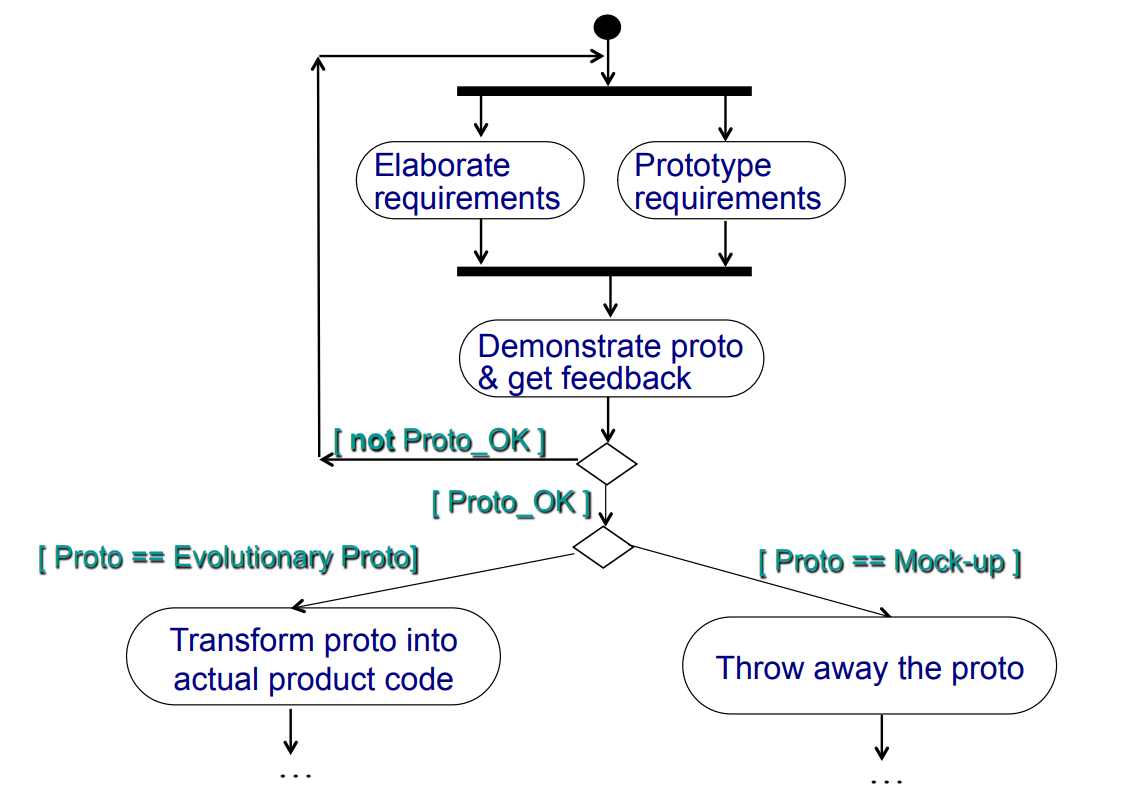
\includegraphics[scale = 0.5]{Imm/flowchartr.PNG}
    \caption{Prototipazione dei requisiti}
\end{figure}
Come pro si ha una sensazione di concretezza per lo stakeholder, anche visuale, permettendo anche già una sorta di training sul software che si produce. Purtroppo spesso i m mock-up sono costosi, inoltre la loro natura simulata può produrre aspettative troppo alte, magari anche solo in termini di prestazioni (il mock-up è super performante mentre il prodotto finale molto meno, avendo tutta la logica applicativa sotto, ad esempio attesa di risposta da un database). Inoltre in un'ottica di riuso un mock-up è spesso inutilizzabile a causa del \textbf{quick-and-dirty code}.

Si ha anche il \textbf{knowledge reuse}, per velocizzare l'elicitation, riusando conoscenze pregresse da sistemi simili a quello sotto studio.\\
Si hanno 3 fasi:
\begin{enumerate}
  \item \textbf{retrieve}: trarre conoscenze e informazioni rilevanti da altri sistemi
  \item \textbf{transpose}: riportare le conoscenze acquisite nel sistema in studio
  \item \textbf{validate, adapt, integrate}, ovvero convalidare il risultato, adattarlo se necessario e integrarlo con la
  conoscenza del sistema già acquisita
\end{enumerate}
Le conoscenze possono essere dipendenti o indipendenti dal dominio.\\
Per quelle indipendenti dal dominio viene utilizzata una tassonomia presente nella slide 26. La tassonomia abbiamo visto che veniva rappresentata attraverso un albero, per ogni nodo o foglia ci poniamo nell'ottica di chiederci se, dal requisito rappresentato nel nodo, possiamo ricavare requisiti di istanza. \\
Sia ad esempio preso in cosiderazione il tempo di risposta, possiamo chiederci: tempo di risposta per cosa? partecipanti? notifica di un meeting?\\
Per quelle dipendenti dal dominio quello che facciamo è eseguire la specializzazione trasformando gli oggetti astratti in oggetti concreti all'interno del sistema. 

Si hanno i seguenti pro:
\begin{itemize}
  \item analisti esperti riutilizzano naturalmente dall'esperienza passata
  \item riduzione degli sforzi di eliciation
  \item ereditarietà della struttura e qualità delle specifiche del dominio astratto 
  \item efficace per completare i requisiti con aspetti trascurati
\end{itemize}
e i seguenti contro:
\begin{itemize}
  \item efficace solo se il dominio astratto è sufficientemente simile e  accurato 
  \item definire domini astratti per una riusabilità significativa è difficile 
  \item si hanno forti sforzi di convalida e integrazione 
  \item le corrispondenze vicine possono richiedere adattamenti complicati
\end{itemize}

Ci sono altri metodi artefact-driven:
\begin{itemize}
    \item \textbf{Card Sort}, si chiede agli stakeholders di posizionare i cartoncini che rappresentano concetti, in modo testuale o grafico. Si chiede poi di classificarli per somiglianza all'interno di un subset, usando i loro criteri di valutazione.(es: sotto un subset "Fitness" associamo i cartoncini "Workout", "Hydration") \\ Per ogni subset viene chiesto le proprietà utilizzate per il raggruppamento. Questo viene eseguito in modo iterativo per nuovi gruppi/nuove proprietà. Come obiettivo vogliamo acquisire nuove informazioni sul concetto già appreso. 
    \item \textbf{Data collection} avevamo detto che si usano dati di marketing, e come obiettivo quello di raccogliere fatti e figure. Questo viene fatto attraverso l'uso dei dati che sono esposti pubblicamente dall'azienda. 
\end{itemize}

\subsubsection{Stakeholders-driven}
Passiamo quindi alle tecniche in cui interagisce direttamente lo stakeholder, senza la mediazione di artefatti.\\
La principale tecnica è l'\textbf{intervista} che consiste in:
\begin{itemize}
  \item selezione mirata dello stakeholder, in base alle informazioni necessarie
  \item fare l'intervista registrando le risposte
  \item scrivere il \textit{transcript} dell'intervista e produrre subito il report
  \item sottomettere all'intervistato il report per validazione
\end{itemize}
Si può avere un'intervista anche con più stakeholder (perdendo però in parte la costruzione del rapporto personale con lo stakeholder). L'intervista è una tecnica costosa e le interviste possono essere poche, bisogna quindi procedere in modo attento.\\

Si hanno due tipi diversi di interviste:
\begin{enumerate}
  \item \textbf{interviste strutturate}, dove si parte con un insieme di domande già scelto per un certo obiettivo. Si da poco spazio ad una discussione aperta
  \item \textbf{interviste non strutturate}, dove si da spazio alla discussione aperta e libera sul \textit{system-as-is}, sulle problematiche e sulle possibili soluzioni. 
\end{enumerate}
Spesso si hanno interviste miste, nella prima parte strutturate e poi con domande e argomenti liberi. Gli argomenti vanno calibrati così come il numero di domande, per evitare perdite di tempo e di perdità di concentrazione da parte dello stakeholder.\\
Vediamo quindi qualche linea guida per la preparazione delle interviste.
\begin{itemize}
  \item bisogna arrivare preparati, tramite il background study, evitare domande ovvie per l'intervista.
  \item per costruire un rapporto con lo stakeholder le domande devono essere su  misura dello stesso, in base al suo lavoro e ruolo
  \item mettere in centro all'intervista necessità e problematiche dell'intervistato, chiarendo di essere interessati al suo punto di vista
  \item evitare che la discussioni dilaghi su argomenti inutili
  \item fare in modo che l'intervistato si senta a suo agio, magari iniziando con qualche chiacchiera informale e domande semplici per poi spostarsi su domande difficili
  \item dimostrarsi affidabile
  \item chiedere sempre perché qualcosa vada fatto, questo per conoscere la motivazione che ha lo stakeholder riguardo la creazione del applicativo
  \item evitare domande bias che influenzino la risposta
  \item evitare domande a cui sicuramente l'intervistato non sa rispondere
\end{itemize}

Nel transcript bisogna includere reazioni personali (anche se queste parti possono essere tolte dalla copia di validazione).\\
Si hanno modi alternativi per interagire con lo stakeholder. Talvolta si ha bisogno anche di altre modalità oltre la sola intervista.\\
Spesso è più facile infatti far osservare che descrivere a parole e quindi si hanno \textbf{studi osservazionali e etnografici}, ovvero studi che si basano sull'osservazione degli stakeholders all'azione osservando come svolgono vari task per cogliere problemi e funzionalità. Si hanno due modalità di osservazione:
\begin{enumerate}
  \item \textbf{osservazione passiva}, dove non si produce interferenza sulle azioni dello stakeholder, guardando da fuori, registrando record e producendo un transcript. Si hanno due particolari \textbf{osservazioni passive}:
      \begin{enumerate}
        \item \textbf{protocol analysis}, dove si osserva qualcuno che svolge un certo task (la slide dice che viene contemporaneamente spiegato)
        \item \textbf{ethnographic studies}, studio che si svolge in un lungo periodo di tempo, dove si prova a scoprire le proprietà emergenti del gruppo sociale coinvolto
      \end{enumerate}
  \item \textbf{osservazione attiva}, dove si svolge in prima persona i task, diventando eventualmente team member, capendo attivamente come deve essere svolto un task
\end{enumerate}
Gli studi osservazionali aiutano a scoprire requisti che restano altrimenti taciti e a scoprire problemi nascosti, che non si noterebbero nell'intervista. Aiuta anche a contestualizzare le informazioni. È comunque un'operazione lenta e costosa, dovendo recarsi di persona ad osservare ed annotare. Può essere potenzialmente inaccurato in quanto una persona conscia di essere osservata potrebbe comportarsi in modo diverso. L'osservazione si focalizza comunque solo sul \textit{system-as-is} e non aiuta molto nel \textit{system-to-be}.\\

Si hanno altri modi di interazione con gli stakeholders tra cui le \textbf{group sessions}, ovvero una famiglia di tecniche utili per la risoluzione di conflitti. L'elicitation prende la forma di un workshop di uno o più giorni in cui si ha una discussione tra vari partecipanti scelti in modo dipendente a seconda dall'obiettivo, innescando una discussione utile a comprendere il \textit{system-to-be}. Mettendo insieme le parti con visioni conflittuali si possono risolvere diversi problemi. Su hanno due tipologie di \textit{group sessions}:
\begin{enumerate}
  \item \textbf{strutturate} dove ogni partecipante ha un ruolo chiaramente definito: leader, moderatore, manager, utente, sviluppatore o altro. Ognuno contribuisce in funzione del ruolo, permettendo di ragionare su requisiti di più alto livello, comuni a più figure, e su conflitti ad alto livello
  \item \textbf{non strutturate}, dette anche \textbf{sessioni brainstorming}, dove i partecipanti non hanno un ruolo definito. La sessione è formata da due fasi:
  \begin{enumerate}
    \item \textbf{generazione delle idee}, dove tutti espongono le proprie idee in merito al problema/conflitto che ha generato la sessione
    \item \textbf{valutazione delle idee}, dove tutte le idee vengono analizzate una per una e valutate per valore, costo, fattibilità e altri parametri da prendere in considerazione in modo da arrivare una visione condivisa sugli approcci da usare secondo una certa prioritizzazione
  \end{enumerate}
\end{enumerate}
Si ha il pro di poter esplorare varie opzioni e a portare a risoluzioni sfruttando anche l'inventiva dei partecipanti. La composizione del gruppo è comunque critica, molti potrebbero non avere tempo, alcuni potrebbero prendere posizioni dominanti introducendo bias, condizionando la discussione e le decisioni. Si rischia inoltre che la discussione diverga verso inutilità senza convergere sugli aspetti per cui è stata convocata la sessione.\\ \textbf{Ogni attività, sia artefact-driven che stakeholder-driven viene svolta solo se si hanno chiari gli obiettivi che si vogliono ottenere con tale attività.}

\section{Evaluation \& agreement}
\subsection{Requirements evaluation}
Ci sono alcuni aspetti che definiscono in modo concerto come valutare i requisiti in maniera rigorosa. Vediamo i punti caratterizzanti della fase di valutazione degli requisisti:
\begin{itemize}
  \item \textit{inconsistency management}, quindi identificazione e risoluzione delle inconsistenze. Questi potrebbero corrispondere, ad esempio, alla gestione conflittuale di due punti di vista differenti da parte di due stakeholders al fine di trovare un accordo. Quello che comprende sono:
  \begin{itemize}
    \item tipi di inconsistenza
    \item gestione delle stesse 
    \item gestione dei conflitti in modo sistematico
  \end{itemize}
  \item la valutazione di alternative per prendere decisioni, una tecnica da adottare potrebbe prevedere la selezione dell'alternativa "preferita".
  \item la prioritizzazione dei requisti, \textit{requirements prioritization}; usata per risolvere conflitti, porre vincoli per costi/tempistiche. Fase che inoltre è intenta a supportare lo sviluppo incrementale.
\end{itemize}

\subsubsection{Inconsistency management}
Definiamo \textbf{inconsistenza} come la violazione della regola di coerenza tra gli elementi, le inconsistenze sono molto frequenti nell'ambito del requirments engineering e si ha una distinzione dei tipi di incosistenza: 
\begin{itemize}
    \item \textbf{inter‐viewpoints}, quando ogni stakeholder ha il suo obiettivo primario e diverse preoccupazioni a riguardo, ad esempio uno stakeholder del dipartimento di marketing avrà obiettivi e altre valutazioni da effettuare rispetto ad un esperto del dominio applicativo.
    \item \textbf{intra‐viewpoints}, quando si hanno conflitti tra i requisti di qualità (qualitativi) (conflitti per esempio tra sicurezza e accessibilità)
\end{itemize}
Le in devono identificate e risolte, dal punto di vista dei tempi:
\begin{itemize}
  \item \textit{non troppo presto}, per avere prima un'elicitation più approfondita 
  \item \textit{non troppo tardi}, per permettere lo sviluppo del software, questo perché ci si potrebbe ritrovare con un prodotto dove qualsiasi cosa può essere stata sviluppata da specifiche incoerenti.
\end{itemize}

Possiamo distinguere diverse tipologie di inconsistenza:
\begin{itemize}
  \item \textbf{terminology clash}, avendo lo stesso concetto denominato diversamente in statement diversi. 
  \item \textbf{designation clash}, avendo lo stesso nome per concetti diversi in statement diversi
  \item \textbf{structure clash}, avendo lo stesso stesso strutturato in modo diverso in statement diversi
\end{itemize}

Distinguiamo inoltre:
\begin{itemize}
  \item \textbf{conflitto forte}, avendo statement non soddisfacibili contemporaneamente (ad esempio $S\land \neg S$)
  \item \textbf{conflitto debole (\textit{divergenza})}, avendo statement non soddisfacibili contemporaneamente in certe condizioni e con certi vincoli
\end{itemize}

Per gestire i clash (scontri) in termini di terminologia, designazione dei compiti e struttura si usa il glossario costruito nella fase di elicitation (dove vengono anche usati eventualmente acronimi).\\
In entrambe le due classi, debole e forte, dei conflitti più sono difficili da gestire, più profonde(grandi) sono le cause (danni) generate, identifichiamo come cause:
\begin{itemize}
  \item obiettivi personali in conflitto da parte degli stakeholder. Questa cosa che andrebbe gestita alla base propagandone i risultati al livello dei requirements
  \item legati ad alcune preoccupazioni di natura non funzionale, come ad esempio prestazioni vs sicurezza. Questa cosa che andrebbe gestita tramite uno studio dei tradeoff, i compromessi, migliori
\end{itemize}

\subsection{Gestione dei conflitti}

Come detto la gestione dei conflitti avviene in modo sistematico seguendo i punti denominati nel schema:
\begin{figure}[H]
    \centering
    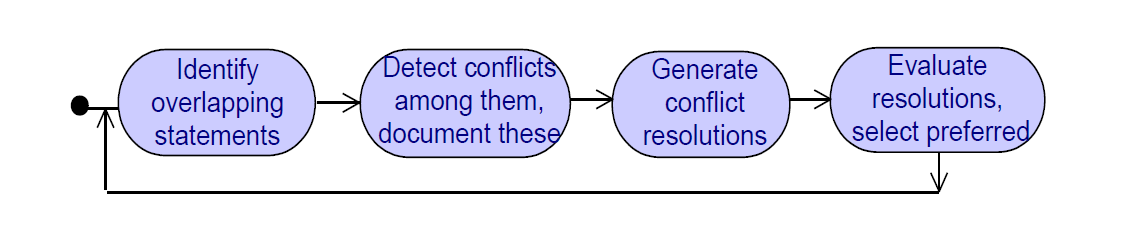
\includegraphics[scale = 0.5]{Imm/manage_conflicts.PNG}
\end{figure}
\begin{itemize}
    \item Identificare di sovrapposizione degli statements, fa riferimento a termini o fenomeni comuni. Si potrebbero assumere delle precondizioni per dichiarazioni contrastanti.
    \item La seconda fase corrispondente al rilevamento dei conflitti, può essere fatto informalmente, tramite euristiche sulle categorie dei requisiti in conflitto, o formalmente. \\
    Conflitti rilevati dovrebbero essere documentati per una successiva risoluzione e analisi dell'impatto. Si usano strumenti come l'\textbf{interaction matrix} che presenta su righe e colonne gli statement e negli incroci indica: 
    \begin{itemize} 
        \item 1 per il conflitto 
        \item 0 per nessun overlap 
        \item 1000 per overlap senza conflitto 
    \end{itemize} 
    Avendo, per ogni statement $S_i$, indicando con $S_i$ la riga/colonna corrispondente (sono uguali):\\
    $conflict(S_i)= \displaystyle \left(\sum_{s\in S_i}s\right) \mod 1000\quad$ e 
    $\quad nonConflictingOverlaps(S_i)=  \displaystyle \Bigl\lfloor{ \left(\sum_{s\in S_i}s \right) } \// {1000}\Bigr\rfloor$
    \item La terza fase, quando generiamo una soluzione ai conflitti riscontrati, per migliori risultati sarebbe meeglio:
        \begin{itemize}
            \item considerare e valutare \textbf{PRIMA} più soluzioni possibili, queste solo le soluzioni candidate ad essere le migliori
            \item confrontare, selezionare (o concordare) quale sia la migliore/la preferita \textbf{DOPO}
        \end{itemize}
    Teniamo ben presente che la generazione delle soluzioni candidate vengono generate tramite tecniche di elicitation e usando tattiche di risoluzione dei conflitti, quali:
        \begin{itemize}
          \item evitare condizioni con limite imposto 
          \item ripristinare statement in conflitto
          \item indebolire gli statement in conflitto
          \item non considerare statement a bassa priorità
          \item approfondire source e target del conflitto
        \end{itemize}
     \item Quarta fase prevede l'uso di vari criteri per la scelta della soluzione migliore/preferita, questi criteri sono:
        \begin{itemize}
            \item contributo a requisiti non funzionali critici 
            \item contributo alla risoluzione di altri conflitti e rischi 
            \item applicazione dei principi di \textit{risk analysis}
        \end{itemize}
\end{itemize}
\subsection{Requirements Prioritization}
Ai vari requisti (elictred e valutati) va imposta una prioritizzazione in termini di:
\begin{itemize}
  \item risoluzione dei conflitti 
  \item limitazioni delle risorse (budget, personale, programmi) 
  \item sviluppo incrementale 
  \item ripianificazione a causa di problemi imprevisti
\end{itemize}
Alcuni principi che vengono utilizzati per una prioritizzazione efficiente sono:
\begin{enumerate}
  \item ottenere pochi livelli ordinati di uguale priorità
  \item utilizzare livelli relativi ("maggiore di" etc$\ldots$) 
  \item avere requisiti comparabili: stessa granularità, stesso livello di astrazione 
  \item utilizzare requisiti non mutuamente dipendenti (uno può essere mantenuto, un altro eliminato) 
  \item tramite un'accordo con i vari partecipanti e stakeholder
\end{enumerate}
Per i primi tre posso usare una tecnica sistematica basata su diversi step:
\begin{itemize}
  \item stimare il contributo relativo di ogni richiesta al \textbf{valore} del progetto 
  \item stimare il contributo relativo di ciascuna richiesta al \textbf{costo} del progetto 
  \item tracciare il \textbf{diagramma valore-costo}
\end{itemize}
\begin{figure}[H]
    \centering
    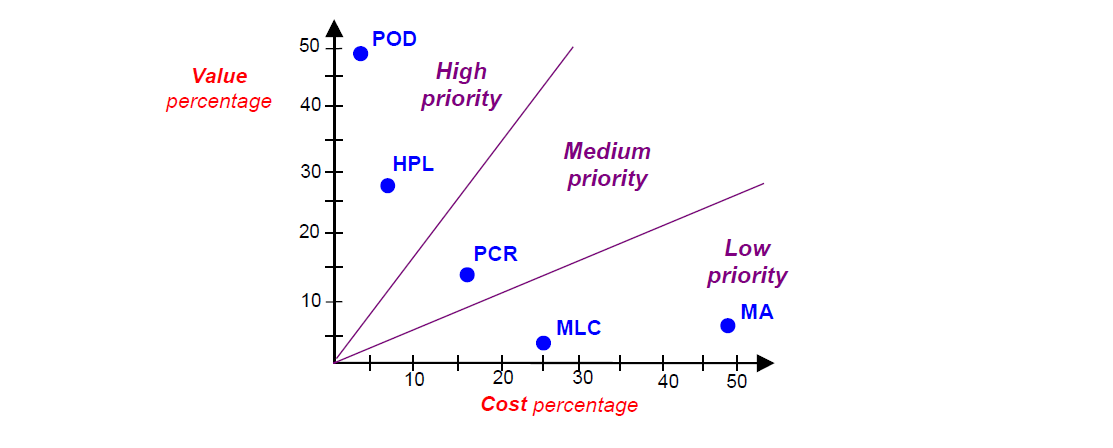
\includegraphics[scale = 0.5]{Imm/plot.PNG}
\end{figure}

Si usa quindi la tecnica AHP dalla \textbf{Decision Theory} dove si cerca di determinare in che proporzione ogni requisito $R_i$, con $i = 1, \dots, N$, contribuisce al criterio $Crit$. Il crietrio $Crit$ viene applicato due volte; la prima volta in funzione del \textbf{Valore}, $Crit=value$, e poi per il \textbf{costo}, $Crit=cost$.\\
Si hanno quindi due step:
\begin{enumerate}
  \item Costruire la \textbf{comparison matrix}, questo ci aiuta a stimare quanto il i-esimo requisito $R_i$, contribuisce al criterio, quando messo a confronto con il j-esimo requisito $R_j$
  \item Determinare come il criterio $Crit$ si distribuisce all'interno di tutti i requisiti $R_i$
\end{enumerate} 

Avevamo detto di utilizzare \textbf{AHP} per il confronto. Questa tecnica esegue 2 step, che prima vengono eseguiti con criterio "Value" e alla seconda iterazione con criterio "cost":
\begin{enumerate}
    \item Confronta i requisiti a coppie. Per poterlo fare inizialmente si usa matrice. Ogni elemento $R_{ij}$ della matrice rappresenta l'importanza del i-esimo criterio relativo al j-esimo criterio. Se il valore $R_{ij}$ è maggiore di 1, ci indica che i-esimo criterio è più importante del j-esimo. L'importanza viene concordata su una scala da 1 a 9. Quindi se il valore di $R_{ij}$ è: 
        \begin{itemize}
            \item 1, allora $i$ e $j$ sono equamente importanti
            \item 3, allora $i$ è poco più importante di $j$
            \item 5, allora $i$ è più importante di $j$
            \item 7, allora $i$ è molto più importante di $j$
            \item 9, allora $i$ è definitivamente più importante di $j$
        \end{itemize}
        All'interno della matrice i valori di $R_{ji} =\displaystyle \frac{1}{R_{ij}}$
    \item Nella seconda parte viene valutato come il criterio si distribuisce all'interno di tutti i requisiti. Si costruisce quindi la matrice che ci permette di effettuare sempre un confronto a coppie, ma con valori normalizzati. Normalizzati perché la somma delle colonne corrisponde a $1$. Ogni colonna è calcolate come: $$\overline{R_{ij}} = \displaystyle\frac{R_{ij}}{\sum_i(R_{ij})}$$ Il contributo del requirment è quindi poi dato eseguendo la media sulle righe:
    $$Contrib(R_j, Crit) = \frac{\sum_i(\overline{R_{ij}})}{N}$$
\end{enumerate}
\section{Specification $\&$ documentation}
In questa fase si documentano in modo preciso i requisiti scoperti. Si descrivono in modo preciso le feature e i concetti rilevanti per il progetto. Nel dettaglio si definiscono in modo preciso:
\begin{itemize}
  \item obiettivi, concetti, proprietà di dominio rilevanti, requisiti di sistema/software, ipotesi, responsabilità 
  \item il che cosa c'è dietro a certe decisioni, quindi la ragione (razionale)
  \item un'indicazione sulle varianti e sulle evoluzioni previste
\end{itemize}
Il documento deve avere una struttura coerente. La documentazione del tutto in un formato comprensibile a tutte le parti, mettendo in allegato i costi, il piano di lavoro e i tempi di consegna del risultato. Il documento in output di questa fase  è detto \textbf{requirements Document (\textit{RD})}. Qualora i requisti siano stati messi online si procede alla costruzione di un db che tiene traccia di tutti i requisti. 

In ogni caso il contenuto deve essere accessibile e comprensibile da tutte le parti interessate, aggiungendo spesso in allegato anche costi, workplan e piani di delivery. Bisogna capire come effettivamente documentare i requisiti.\\ La prima opzione è l'utilizzo del linguaggio naturale in modo svincolato, in prosa. Si ha una forte espressività ma, in assenza di regole sulla scrittura si rischia di produrre una sorta di romanzo, producendo qualcosa di poco gestibile. Il linguaggio naturale inoltre può nascondere ambiguità (basti pensare anche solo a sequenze di \textit{or} e \textit{and}, non si sa come andare a combinare queste sequenze non avendo una tabella di verità utile per confronto). Usando il linguaggio naturale privo di vincoli si hanno quindi rischi, esiste una pratica più ragionevole, ovvero usare un \textit{linguaggio naturale strutturato}. Si introducono quindi due tipi di regole:
\begin{enumerate}
  \item \textbf{local rules}, che riguardano la scrittura del singolo requisito
  \item \textbf{global rules}, che riguardano le regole sulla scrittura dell'intero documento e sull'insieme dei requisti
\end{enumerate}
Bisogna però introdurre alcune regole stilistiche generali (le stesse che si dovrebbero applicare anche per una tesi):
\begin{itemize}
  \item scrivere pensando a chi deve leggere, il modo in cui scriviamo e il livello di astrazione, con il quale affrontare il discorso, viene valutato anche in base al interlocutore. Infatti questo deve essere ben identificato.
  \item spiegare cosa stiamo per scrivere prima di specificarlo nel dettaglio
  \item prima motivare le scelte, indicare le scelte e poi fare un sintesi di queste ultime
  \item assicurarsi che ogni concetto usato nei requisiti sia stato ben definito 
  \item chiedersi se quanto scritto è comprensibile e rilevante (per capirlo basta cancellare quanto scritto e vedere se si capisce ancora)
  \item non esporre più di un requisito, assunzione o una proprietà del dominio all'interno di una singa frase. Scrivere frasi brevi
  \item distinguere ciò che è obbligatorio e deve essere implementato, da ciò che si potrebbe implementare qualora si volesse
  \item evitare acronimi non necessari ed evitare l'abuso del gergo informatico
  \item usare esempi esplicativi per meglio chiarire i concetti indicati
  \item usare diagrammi o illustrazioni quando possibile
\end{itemize} 
In termini di \textbf{local rules} si hanno dei template per scrivere i requisiti, usando anche un solo standard per tutti i requisti. Un esempio di template che si potrebbe utilizzare per la stesura dei requisiti potrebbe essere il seguente:
\begin{itemize}
  \item identificatore del requisito (con uno schema di naming significativo, magari con uno schema gerarchico con combinazioni di caratteri tramite separatore per specificare al meglio il requisito)
  \item indicare la categoria di appartenenza del requisito (funzionale, assunzione etc$\ldots$)
  \item specifica del requisito, questo significa che deve seguire alcune le regole stilistiche
  \item criterio di fit (una sorta di test di accettazione, usato quindi per quantità/concetti misurabili, essendo critico quindi per requisiti non funzionali) 
  \item fonti di elicitazione che hanno portato alla elicitation di quel requisito
  \item la ragione per cui quel requisiit esiste (razionale)
  \item interazioni con altri requisti (contribuzioni, dipendenze e conflitti)
  \item stabilire il livello di priorità
  \item livelli di stabilità (per indicare le chance di cambiamenti)
\end{itemize}

Per le \textbf{global rules} si ha una forma standard data da \textbf{IEEE std-830}, il più diffuso. Si hanno varie macrocategorie a loro volta suddivise:
\begin{enumerate}
  \item Introduzione (dove si specifica anche quale parte del documento interessi ai vari stakeholder)
  \begin{enumerate}
    \item motivazioni del documento
    \item scopo del prodotto, una sua breve descrizione: contiene il dominio, lo scopio e l'obiettivo del system-to-be
    \item definizioni, acronimi, sigle e abbreviazioni
    \item reference, quali sono le fonti di elicitazione
    \item overview dell'organizzazione del documento
  \end{enumerate}
  \item Descrizione generale, è importante definire quale sia il confine tra il prodotto che viene realizzato e l'ambiente in quale esso interagisce. 
  \begin{enumerate}
    \item prospettive del prodotto
    \item funzionalità principali
    \item caratterizzazione degli utenti
    \item vincoli generali sull'ambiente (che non possono esse modificati ma con i quali si deve integrare il prodotto)
    \item assunzioni sul prodotto e dipendenze del prodotto
    \item ripartizione dei requisti
  \end{enumerate}
  \item Requisiti specifici, i requisiti vengono indicati con il massimo livello di dettaglio facendo uso di un template. (spesso questa fase è molto importante per gli sviluppatori). Si hanno quindi varie categorie di requisiti che articolano le varie sezioni del capitolo:
  \begin{enumerate}
    \item requisiti funzionali (che a sia volta un'organizzazione interna in base a vari fattori, come aree funzionali, componenti etc$\ldots$)
    \item requisiti per l'interfaccia esterna
    \item requisiti per le prestazioni
    \item vincoli di progettazione
    \item attributi di qualità del software
    \item altri requisiti
  \end{enumerate}
  \item appendice, questo solo c'è qualcosa da allegare al suo interno, possiamo anche omettere questa fase se non si hanno informazioni utili da aggiungere.
  \item indice
\end{enumerate}

Si hanno anche opzioni aggiuntive oltre al linguaggio naturale. Si puo fare uso di diagrammi, avendo quindi una \textbf{notazione semi-formale}. Significa che il diagramma ha una sintassi formale essendo i vari diagrammi formalmente definiti ma interpretazione degli stessi può comunque essere ambigua.\\
I diagrammi sono utili per complementare quello che abbiamo scritto in linguaggio naturale, che risulta spesso troppo complesso e articolato. Un diagramma può semplificare quanto scritto e rappresentare il tutto in modo compatto. L'uso di diagrammi permette di comunicare più semplicemente e viene usato per aspetti specifici del sistema. Facciamo comunque attenzione all'aspetto semi formale che porta con se una certa ambiguità. Si ha quindi la stessa ambiguità di interpretazione che si aveva nei linguaggi naturali\\ 
\subsection{Tipologie di diagrammi}
\textbf{Problem diagram} questo tipo di diagramma descrive i requisiti a livello di sistema. Si mostrano le componenti del sistema dove ogni componente è indicato tramite un rettangolo con doppia linea verticale. Il sistema comunica con diversi elementi dell'ambiente, indicati da rettangoli. Il diagramma ci permette di specificare un requisito nella forma testuale, e riferire questo requisito agli elementi dell'ambiente. Posso avere, oltre che dei riferimenti, dei vincoli che si pongono su elementi a partire dal requisito.\\
Tutte le interazioni sono decorate con gli eventi che sono rilevanti per l'interazione con il produttore dell'evento. All'interno del diagramma indichiamo: \textbf{Componente sistema} \textbf{$!$}  \textbf{Evento che il componente produce}.\\
Con questo tipo di diagramma si cattura il contesto del requisito, legandolo  componenti dell'ambiente e componenti del sistema, tramite specifici eventi. Si identificano a colpo d'occhio gli elementi rilevanti per un certo requisito. Esistono dei pattern che catturano i problemi più frequenti in modo da facilitare la creazione di un Diagram. Questi prendono il nome di Frame Diagrams. Quello che possimao tirare dai pattern sono:
\begin{itemize}
    \item tipo di componente (indicato con un quadratino in basso a destra nel rettangolo della componente) specificato da una lettera:
        \begin{itemize}
            \item C: causal, causa-effetto
            \item B: biddable, non predicibile
            \item X: lexical, lessicale, specifica artefatti
        \end{itemize}
    \item tipo di evento, posto dopo il ! sopra descritto, specificato da una lettera: 
        \begin{itemize}
            \item C: causal, diretta conseguenza di altri eventi
            \item E: event, che non sono diretta conseguenza ma che sono prodotti in modo spontaneo 
            \item X: lexical, dati che vengono utilizzati per produrre qualcosa
        \end{itemize}
\end{itemize}
I pattern vengono istanziati nei vari casi specifici. 

Abbiamo inoltre il \textbf{Context diagram} che dichiara le componenti del sistema e le loro interfacce, quindi di conseguenza anche la struttura del sistema, cosa è presente nel sistema e cosa gli è esterno e l’ambiente di ogni componente (vicini, interfacce).\\

Un altro diagramma tipico è quello \textbf{ER} che ci permette di specificare quale sono le entità che entrano in gioco in particolari aspetti dei nostri requisiti, specificando tutto in modo schematico.\\
Si usano anche diagrammi di dominio, di classe etc$\ldots$, non descrivendo più comportamenti ma strutture, domini etc$\ldots$\\

Un altro tipo di Diagrams sono i \textbf{SADT diagrams} che si dividono in due tipi, e permettono di specificare il comportamento di alcune attività che un sistema software deve seguire, scomponendo questo ultimo e aggiungendo varie informazioni. Questi diagrammi possono essere activity-driven o data-driven.
\begin{enumerate}
    \item actigram, di tipo activity-driven, si concentra sulle attività e mostra le dipendenze tra attività in termini di dati. 
        \begin{itemize}
            \item East$\longrightarrow$ per l'input di dati
            \item West $\longrightarrow$ per l'output di dati
            \item North $\longrightarrow$ per il data/event controlling, ovvero dati o eventi che controllano il comportamento dell'attività
            \item South $\longrightarrow$ per l'unità che processerà l'attività (opzionale)
        \end{itemize}
    \item datagram, di tipo data-driven, si concentra sui dati e mostra le dipendenze tra dati in termini di attività.
        \begin{itemize}
            \item East $\longrightarrow$ per l'input di attività che producono il dato
            \item West $\longrightarrow$ per indicare attività le quali devono utilizzare il dato
            \item North $\longrightarrow$ per le attività di validazione del dato
            \item South $\longrightarrow$ per le risorse necessarie a memorizzare e gestire il dato
        \end{itemize}
\end{enumerate}
Le attività sono indicate dentro rettangoli e si hanno una serie di frecce che a seconda della direzione variano il significato, noi abbimao usato \textbf{Norh} e \textbf{West}, andrebbe usato $\uparrow$, $\longleftarrow$.\\
La coerenza tra di due diagrammi è fondamentale avendo una rapporto di \textbf{dualità} tra essi quindi i dati e le attività presenti in uno devono apparire anche nell'altro.\\
Questo strumento, ovvero il diagramma di tipo \textbf{SADT}, si prestano a documentare workflow molto semplici. In ogni caso:
\begin{itemize}
    \item ogni attività \textbf{DEVE} avere un input e un output 
    \item tutti i dati devono avere un produttore e un consumatore 
    \item i dati I/O di un'attività devono apparire come dati I/O delle sottoattività 
    \item ogni attività in un datagramm deve essere definita in un actigramma
\end{itemize}

Abbiamo poi il \textbf{Dataflow diagram}, diagrammi che catturano le operazioni del sistema collegate per mezzo delle dipendenze tra dati (sono più semplici ma meno espressivi degli actigram).\\
Un’operazione è un’attività di trasformazione sui dati. I collegamenti di input e di output sono i flussi si dati: le operazioni necessitano di un flusso di dati in entrata per produrre un flusso di dati in uscita.\\
La regola di trasformazione dei dati deve essere specificata nelle annotazioni in linguaggio naturale strutturato o in un altro DFD (dataflow diagram).\\
I componenti del sistema e le repository di dati sono l’origine e la fine dei flussi.
Il soddisfacimento delle regole di consistenza e completezza può essere controllato mediante appositi strumenti.    \\

Un altro diagramma classico è il \textbf{case use diagram} per visualizzare i requisiti identificati, che prendono forma di casi d'uso con gli attori che partecipano allo svolgimento dei requisiti. Si possono mostrare diversi tipi di relazioni, come ad esempio le inclusione o le estensioni.\\

Un altro strumento utile nella definizione di workflow è l'\textbf{event trace diagrams}, ovvero i diagrammi di sequenza. Se ne hanno vari tipi con sintassi più o meno ricche ma in generale si hanno $N$ elementi che partecipano all'esecuzione che viene mostrata visualmente. Si possono inolre mostrare varie richieste e risposte, sincrone o meno, che vengono indicate cronologicamente dall'alto al basso. Questa visualizzazione compatta aiuta nel momento in cui il linguaggio naturale diventa troppo complesso per spiegare una certa sequenza di azioni. \\

Un altro diagramma usato è il \textbf{state machine diagram} per mostrare in quali stati un particolare elemento si trova e quali transizioni/eventi modificano i suoi stati. Questi diagrammi sono utili in quanto in modo compatto rappresenta il ciclo di vita di una certa componente, facilitando la creazione del sistema. \\

\textbf{Statechart}: composizione parallela di diagrammi state machine, uno per ogni variabile che si evolve in parallelo. I componenti spesso controllano diversi item in parallelo. Il problema dei diagrammi $StateMachine$(SM) era che per $N$ variabili (item) ognuno con $M$ possibili valori sarebbero stati necessari $M^N$ stati; per cui alcuni stati degli SM mischiano diverse variabili. Uno stato di uno statechart invece rappresenta l’aggregazione di sottostati correnti e per $M^N$ stati di $SM$ servono solo $M \cdot N$ stati per statechart.\\
\textit{Semantica interleaving}: se si hanno due transizioni che dovrebbero scattare dallo stesso stato, vengono eseguite in maniera sequenziale (scelta non deterministica).\\

Come altro diagramma abbiamo il \textbf{R-net diagram} che permette di mostrare come reagisce un sistema in base ad un certo stimolo. È un albero che parte con uno stimolo, dopo il begin, posto in un esagono e si sviluppa in base alle varie alternative in corrispondenza di punti di decisione ($\bigoplus$). Nei rettangoli si hanno le azioni che sono svolte in conseguenza allo stimolo.\\

I diagrammi sono tra loro complementari ma hanno anche delle intersezioni tra loro e anche con il testo e tutto deve comunque restare coerente. Si rischia di introdurre inconsistenze. Quando lavoriamo con i diagrammi, visto che abbiamo una sintassi formalmente definita seppure con una semantica ambigua, ci sono alcune regole di consistenza che alcuni strumenti possono applicare per noi.\\

Uno degli standard per la modellazione di diagrammi è il: \textbf{Unified Modeling Language (\textit{UML})}. Al suo interno si hanno, con regole di coerenza tra essi:
\begin{itemize}
  \item class diagrams
  \item use case diagrams
  \item sequence diagrams
  \item state diagrams
\end{itemize}

In conclusione i diagrammi hanno il pro di essere in grado di dare una buona panoramica e struttura/comportamento, facile da trasmettere e comprendere, di aspetti importanti. Sono inoltre supportati da vari tool di analisi. L'elemento debole resta la semantica ambigua che ci limita anche nell'analisi dei diagrammi stessi.\\

Il modo delle notazioni formali, in modo da ottenere oltre a una sintassi formale anche una semantica formale. Questi tipi di linguaggi vengono usati per sistemi critici, questo per via del alto costo che comportano.

\subsection{Notazioni formali}
Si parla sia di sintassi che di semantica formalmente definite. Tali definizioni formali permettono che il compilatore sia in grado di processarle completamente: viene infatti formalizzata sia la parte dichiarativa (la struttura dell’item come per i diagrammi), la parte assertiva (le proprietà degli item) e i meccanismi per strutturare ampie specifiche in unità più piccole. La loro definizione formale è espressa spesso tramite la logica matematica e vengono definite la sintassi, la semantica e le regole di inferenza per le nuovi informazioni.\\
Si ha quindi un livello di precisione alto e non si ha ambiguità, permettendo analisi di consistenza e coerenza dei requisiti (fatta direttamente dal calcolatore).\\

Una sintassi/semantica formale è quella data dalla logica proposizionale e dalle \textbf{formule ben formate}. Si ha quindi un linguaggio basato sui connettori logici e sulle regole per avere formule ben formate. Ogni statement può quindi essere interpretato con il valore di verità con le regole definite dalla logica e dalle tabelle di verità (ovviamente può farlo il calcolatore).\\
La composizione ricorsiva degli statement non decomponibili attraverso i connettici logici limita l’espressività (non ci sono variabili nè quantificatori).\\
La semantica è definita come segue: \\
L’interpretazione di uno statement è data dagli specifici assegnamenti delle proposizioni atomiche che lo compongono. Il significato di uno statement data un’interpretazione è il valore booleano complessivo dello statement.\\
Regole per inferire nuovi statement da statement già disponibili:
\begin{itemize}
    \item sound rule: se la conclusione è vera per ogni interpretazione che renda vera la premessa.
    \item permettono di derivare automaticamente senza effettuare una valutazione semantica.
\end{itemize}

La logica predicativa del primo ordine permette di estendere l’espressività della logica proposizionale attraverso l’utilizzo di variabili, costanti, quantificatori, relazioni e funzioni.\\
Per quanto riguarda la semantica, l’interpretazione è la definizione di ciò che le variabili non quantificate, le costanti, le funzioni e i predicati designano nel dominio di interesse: le specifiche dei predicati hanno significato solo all’interno della specifica interpretazione.\\
Risulta essenziale documentare le interpretazione per la comunicazione, la non ambiguità e il controllo di adeguatezza, in particolare del dominio di interesse di costanti e variabili non quantificate, funzioni e predicati $n$-ari.

\subsubsection{First-order specification languages}
Abbiamo:
\begin{itemize}
    \item variabili. oggetti designati convolti nei requisiti, nelle proposizioni e nelle assunzioni (entità degli ER)
    \item stato di una variabile: coppia (variabile, valore della variabile) 
    \item stato del sistema: coppia (set di variabili del sistema, set dei corrispondenti valori)
\end{itemize}
In molti linguaggi di specifica, le specifiche sono interpretate sulla base degli stati (le specifiche sono soddisfatte da alcuni stati e falsificate da altri).
Molti linguaggi di specifica di prim’ordine sono ordinati: le typed variable designano alcune istanza in un set.\\
Per specificazione formale si intende un set di statement formali (assiomi) dai quali possono essere derivati altri statement (teoremi) tramite regole di inferenza.
Gli errori di specificazione possono essere: 
\begin{itemize}
    \item contraddizioni: non esiste alcuna interpretazione che rende veri tutti gli statement contemporaneamente..
    \item ridondanza: alcuni statement possono essere derivati da altri.
\end{itemize}
Una derivazione automatica dei teoremi è utile per un controllo di adeguatezza (se si vuole una determinata conseguenza) e un controllo di consistenza (se si riesce a derivare false come teorema).
\subsubsection{Specificazione History-based}
Le specifiche catturano un set massimale di history di sistemi ammissibili. Una history è una sequenza temporale infinita di stati di un oggetto (dichiarati implicitamente: time e history sono mantenuti impliciti).\\
Gli statement sono scritti in una logica temporale (TL) costituita da connettivi logici che si riferiscono a stati passati e futuri. Gli statement TL sono interpretati tramite le history (sono soddisfatti da alcune history e falsificati da altre).\\
Da differenti strutture time/history conseguono differenti TL.
\subsection{Linear Temporal Logic (LTL)}
Si basa su punti discreti del tempo (isomorfi ai naturali), history lineari, connettivi proposizionali e costrutti first-order + connettivi temporali.\\
Si hanno delle estensioni al real-time:
\begin{itemize}
    \item $\diamond_{\leq d}$: più avanti nel futuro all’interno della scadenza $d$
    \item $\ocircle_{\leq d}$ sempre nel futuro fino alla scadenza $d$
\end{itemize}
Si vede quanto produrre tutto questo per un progetto enorme risulti costoso. Si può avere un approccio formale anche usando specifiche basate su stato \textbf{state based specification}, dove definiamo in maniera formale e rigorosa che cosa sono gli stati che il nostro sistema può attraversa e come questi modificano il nostro sistema. \\ Si usano linguaggi come $Z$ basati sulla teoria degli insiemi. Ogni stato è caratterizzato da \textit{pre} e \textit{post} condizioni e si studiano le regole in termini di invarianti che lo stato deve soddisfare.

Sopra si hanno tutti gli elementi coinvolti nell'operazione. Nella parte alta abbiamo le nostre precondizioni e nella parte bassa, sotto di loro, le nostre postcondizioni. Sotto la linea orizzontale abbiamo delle invarianti, che devono essere rispettate.\\

Abbiamo inoltre un modo di rappresentazione delle operazioni. Sopra si hanno tutti gli elementi coinvolti nell'operazione. La prima linea della parte sotto è per le precondizioni, quella sotto per le postcondizioni, entrambe con la notazione insiemistica.\\
I vari elementi che possiamo dichiarare si trovano nella forma sono: 
\begin{itemize}
  \item \texttt{stateVar?:Type} indica una variabile di input
  \item \texttt{stateVar':Type} indica una variabile di output che possono presentare delle modifiche allo stato della variabile
  \item \texttt{stateVar!:Type} indica una variabile di output di tipo esterma, che non permette modifiche di stato
  \item \texttt{$\Delta$ schema} indica che si ha una modifica delle variabili importate dallo schema
  \item \texttt{$\Xi$ schema} indica che non si ha una modifica delle variabili importate dallo schema
\end{itemize}

\subsubsection{Algebraic specification}
La specifica viene rappresentata come equazioni di leggi per la composizione di operazioni e operazioni.\\
Le operazioni vengono viste come funzioni matematiche, non c’è un’esplicata nozione di stata e la storia del sistema è data dalla traccia delle operazioni delle applicazioni.\\
I vantaggi sono un’analisi efficiente e automatizzata, la produzione di specifiche eseguibili, meccanismi strutturali ricchi; di contro, il potere espressivo è limitato (solo equazioni, non ci sono referenze storiche) e si è vicini alla programmazione.\\
   
Quindi per descrivere i requisiti, l’opzione principale è utilizzare il linguaggio naturale strutturato, complementandolo con i diagrammi e utilizzare le notazioni formali sono raramente.
\section{Validation \& Verification}
Ultima fase del nostri ciclo di attività che costituiscono il RE. In questa fase si studia l’RD, ovvero la sua garanzia di qualità, analizzando varie attività:
\begin{itemize}
    \item \textbf{validazione}: quanto contenuto nell’RD dev’essere adeguato con quanto si necessita.
    \item \textbf{verifica}: non ci devono essere omissioni o inconsistenze.
    \item \textbf{correzione}: di eventuali errori e difetti.
\end{itemize}
L'output che si deriva è un documento dei requisiti(RD) consolidato.\\
Si studia durante questa fase quella che è la quality assurance. Ques-  t'ultima si occupa di dare risposta alla domanda \textit{Come faccio a sapere se i requisiti che ho specificato, siano o meno, un coorretto insieme soddisfacente}.\\
Questa domanda ha una risposta molto complessa, questo perché nel caso dei requisiti, chiedersi se un insieme di requisiti specificati è corretto non ha una risposta immedaita.\\
Quello che possiamo fare è utilizzare uno dei seguenti approcci:
\begin{enumerate}
    \item \textbf{Requirements inspection and reviews}: eseguire una ispezione, manuale, dei requisiti prodotti. Vengono analizzati da un team di revisori che cercano specifici tipi di errori all'interno dei requisiti.(più diffuso e più applicabile, può essere ispezionato sempre un requisito, nonché estremamente costoso)\\
    Non possiamo analizzare tutto, dato l'enorme costo che comporterebbe, ma solamente alcune parti che riteniamo più importanti. 
    \item \textbf{Queries on a specfication database}: se i nostri requisiti sono presenti su un database, e se sono ben scritti e ben strutturati, alcuni controlli possono essere automatizzati attraverso delle query che, ad esempio, vanno a verificare se ci sono dei conflitti. L'automazione è parziale, la fase di check è limitata. 
    \item \textbf{Requirements validation by specification animation}: se si sviluppa modellando sin dall'inizio il comportamento del software, possiamo svolgere una attività di sviluppo che continua a utilizzare dei modelli, che man mano vengono concretizzati fino a quando non si arriva alla stesura del codice vero e proprio. Questo codice può essere generato automaticamente dal nostro modello (diagramma). Dato che per alcuni di questi software si possono fare delle verifiche, anche visuali, è possibile individuare dei problemi già nella specifica dei requisiti. 
    \item \textbf{Formal checking}: può rivelare bug sottili, richiede specifiche formali e esperti dei linguaggi formali.
\end{enumerate}

La qualità va assicurata e controllata perché possono esserci errori e difetti nei documenti sui requisiti che possono essere di diversi tipi (omissioni, contraddizioni, ecc) e possono essere i più costosi, numerosi, persistenti e pericolosi errori nel progetto.

Approcci di di verifica della qualità dei requisiti: 

- ispezione e revisione (operazione manuale e costosa in termini di tempo, ma è sempre applicabile)
 
 L’idea base è quella di chiedere a un gruppo di persone di ispezionare individualmente l’RD e successivamente di mettersi d’accordo sui problemi da risolvere.
 Ne esistono forme walkthroughs dove l’ispezione interna viene fatta dai membri del progetto e forme più strutturate dove i valutatori sono esterni, i meeting vengono ben preparati e vengono ispezionati i report. 
 L’ispezione e la revisione sono molto comuni per il source code. 
 Studi empirici hanno mostrato che è processo efficace anche per i requisiti.
 
 1. pianificazione dell’ispezione: determina le revisioni, la tempistica, lo scopo dei meeting e il formato dei report.
 2. revisione individuale: 
    - free mode: non ci sono direttive su dove cercare cosa.
    - checklist-based: si concentra su problemi specifici o su specifiche parti dell’RD.
    - process-based: si assegna un ruolo specifico ad ogni valutatore, comprensivo di procedure specifiche, tecniche di analisi. È il modo più efficace.
 
 Linee guida sull’ispezione:
 
 - il report dell’ispezione dovrebbe essere informativo, accurato, costruttivo (senza opinioni né commenti offensivi).
 - Le ispezioni dovrebbero essere indipendenti dagli autori dell’RD e rappresentative di tutti gli stakeholder quindi avere background differenti.
 - Le ispezioni non dovrebbero avvenire né troppo presto é troppo tardi: meeting più corti e frequenti sono più efficaci.
 - Le ispezioni richiedono una maggiore attenzione per le parti critiche: più difetti ci sono in una parte più richiede attenzione.
 
 Esistono diversi tipi di checklist per l’ispezione il cui obiettivo è guidare la ricerca di difetti verso problemi specifici: 
 
 - *defect-driven*: lista di domande generiche suddivise per tipo di difetto.
 - *quality-specific*: suddivide le domande defect-driven in specifiche categorie NFR (sicurezza, affidabilità, performance, ecc) e si focalizza spesso sulle omissioni.
 - *domain-specific*: ulteriore specializzazione dei concetti di dominio e delle operazioni per rendere ancora più guidata la ricerca dei difetti.
 - *language-based*: specializza la checklist defect-driven ai costrutti specifici del linguaggio e a volte viene parzialmente automatizzata.
 
 Vantaggi: l’ispezione dei requisiti si è verificata più efficace dell’ispezione del codice, ha ampia applicabilità.
 Svantaggi: il processo di ispezione è costoso (per via della dimensione del materiale da ispezionare, perché richiede tempo e costi per gli ispettori esterni e per i meeting e perché non è incrementale) e non c’è garanzia di trovare tutti i difetti.

- query su uno specifico database (parziali, ma automatiche almeno per controlli superficiali)
 
 Sono usate su specifiche diagrammatiche, mantenute nel database dei requisiti (lo schema logico deriva dalla struttura del diagram language).
 Le query catturano i controlli per la consistenza strutturale sia intra- che inter- diagrams, attraverso checklist automatiche di domande.
 Un motore di query diagram-specific può essere generato da un ER meta-spec di un linguaggio di diagramma.
 
 % <img src="C:\Users\alice\AppData\Roaming\Typora\typora-user-images\image-20201125174549137.png" alt="image-20201125174549137" style="zoom:50%;" />
 
 - *press-button mode*: comunemente utilizzata da strumenti CASE, permette di creare query preimpostate per la violazione delle regole. 

- animazioni delle specifiche (parziali e richiede che le specifiche siano eseguibili, ma utile per trovare bug ed è adatto ai non esperti).
 L’obiettivo è di controllare l’adeguatezza dei requisiti rispetto ai bisogni reali.
 
 - approccio 1: mostrare scenari di interazioni concrete in azione.
   Vantaggi: strumento di rappresentazione utilizzabile sui diagrammi ET
   Svantaggi: la copertura dello scenario sul problema.
 - approccio 2: usare tool di animazione per le specifiche
   1. estrarre o generare dalle specifiche modelli eseguibili 
   2. simulare il comportamento del sistema dal modello (sottomettere al modello gli eventi-stimolo per vederne il comportamento di risposta)
   3. visualizzare la simulazione durante l’esecuzione:
      - textual format: comandi inpu, traccia dell’esecuzione
      - diagrammatic: selezione degli eventi di input, processione dei token
      - domain scenes: pannelli di input, scene animate nell’ambiente
   4. ricevere il feedback utente
 
 Si tratta di una modalità model-based per la quale sono disponibili molti animators per i linguaggi di specifica.
 
 Vantaggi: miglior modo per controllare l’adeguatezza rispetto ai veri bisogni e all’ambiente reale, supporta il coinvolgimento degli stakeholder, è estendibile a controesempi animati generati da altri tool e gli scenari animati possono essere tenuti per rivederli più avanti.
 Svantaggi: richiede una progettazione attenta degli scenari che possano mostrare dei problemi, non garantisce la copertura di tutte le inadeguatezze (anche importanti) e richiede delle specifiche formali.

- controllo formale (richiede specifiche formali e esperti; ma può rivelare bug minuziosi)
 
 - language checks (correzione sintattiche, di battitura e di semantica statica)
   Controllo della sintassi in base alle regole grammaticali, controllo dei tipi, controllo della semantica statica (le variabili usate devono essere dichiarate,  inizializzate e utilizzate all’interno di uno certo scope), circularity checking.
 
 - language-specific consistency/completeness check 
   Es. quando i servizi o i comportamenti sono specificati come relazioni I/O, queste relazioni sono funzioni? (per evitare il non determinismo). E nel caso sono funzioni totali? (l’output è specificato per ogni possibile input)
 
 - property verification
   
   - algoritmica (model checking)
     Per verificare se un modello di comportamento soddisfa un requisito, un domain property o un’assunzione, attraverso un’esaustiva ricerca attraverso il modello di un’eventuale property violation.
     La generazione di un controesempio rappresenta una traccia che porta a una violazione.
     Proprietà che possono essere controllate: rechability (la situazione può o non può essere raggiunta), safety (la condizione desiderata è sempre soddisfatta), liveness (la condizione desiderata alla fine verrà soddisfatta)
     
     Vantaggi: controlli completamente automatizzati, ricerca esaustiva (non vien tralasciato alcun eventuale difetto), le tracce dei controesempi possono rivelare errori sottili, difficili da trovare altrimenti, coppia naturale con le animazioni per la visualizzazione delle tracce e sempre più usata dall’industria per i progetti mission-critical.
     Svantaggi: esplosione combinatoria degli stati (attualmente non è utilizzabile per sistemi troppo grandi e perciò utilizzato per il controllo di modelli limitati e astrazioni, perdendo in accuratezza e completezza), i controesempi possono essere complessi e difficili da capire (mostrano i sintomi dei bug e non le cause).
   
   - deduttiva (thereom proving)
     
     Generazione di nuove specifiche formali applicando le regole di inferenza alla logica sottostante.
     Mostrano le conseguenze logiche delle specifiche e evidenziano le incosistenze.
     Sono generalmente interattive per fornire, accettare e rigettare lemmi e suggerire strategie di dimostrazione.
     
     Vantaggi: solidità e completezza del sistema formale usato (ogni conclusione è corretta e ogni corretta conclusione è derivabile), utilizzabile per mostrare specifiche inconsistenti e conseguenze inadeguate, può essere applicato a grandi sistemi (lo spazio infinito degli stati è gestito grazie all’induzione), dimostrazioni fallite possono rivelare la causa di un problema.
     Svantaggi: difficili da usare (richiedono un’alta expertise), non vengono prodotto controesempi.

\section{Requirement evolution} 
Una volta completata la nostra prima iterazione del ciclo RE, quello che facciamo e proseguire eseguendo il prossimo ciclo. Si vede una evoluzione dei requisiti maturando mano a mano il nostro sistema. Sui requisiti vengono ri-eseguite le fasi [1-4].
Come è stato detto queste quattro fasi si ripetono in modo iterativo in modo “a spirale”. Questo viene fatto in quanto si possono avere evoluzioni nel processo nonché correzioni di quanto già fatto che si propagano su tutto il documento. Le evoluzioni e le correzioni possono sopraggiungere durante l’RE stesso, lo sviluppo del software e dopo il deploy del software stesso.\\
Dopo ogni ciclo si è molto più consci del sistema e si può passare al miglioramento del RE con più efficacia. Questo sistema è molto compatibile con i vari metodi agili.\\

Il problem world (problema derivato dal mondo reale) continua a cambiare, e questo crea un impatto sul nostro sistema. Può capitare che cambiano le organizzazioni, i regolamenti, le opportunità, le alternative tecnologiche, evolvono le priorità e i vincoli e con il passare del tempo si ha sempre una migliore comprensione delle caratteristiche del sistema, i suoi punti di forza e i suoi limiti e difetti.\\

Il problema della gestione dell’informazione sorge un quanto bisogna sempre mantenere la consistenza, propagare i cambiamenti e controllare le versioni. Questo problema è mitigato dall’anticipazione del cambiamento e dalla gestione della tracciabilità, quindi tenere traccia dei legami tra i vari requisiti per non genere problemi.\\
La gestione dei cambiamenti nei requisiti è il processo di anticipazione, valutazione, accordo e propagazione dei cambiamenti negli items dell’RD.
\subsection{Prepararsi per i cambiamenti}
Saper distinguere quali requisiti cambieranno di più e quelli sono più stabili e gestire questi in maniera diversa.\\
Identificare i possibili cambiamenti, accertarne la probabilità e documentarli serve per anticipare un’adeguata risposta per quando il cambiamento avverrà e per progettare un’architettura che rimanga stabile a prescindere dai cambiamenti.\\
Per farlo, si associano livelli di stabilità, caratterizzati da gruppi di statement suddivisi per caratteristiche, ai nostri requisiti. Questo ci permette di gestire cambiamenti diversi in base alla tipologia dei requisiti.\\ Si usa un piccolo numero di livelli, ognuno contenente item di pari stabilità.
I livelli di stabilità sono un metodo di confronto tra requisiti qualitativo e relativo.\\
Nel livello di stabilità più alto si trovano le feature che vengono mantenute in qualsiasi contrazione, estensione o variante del sistema.
Aspetti intenzionali e concettuali e aspetti funzionali che incontrano obiettivi chiavi sono più stabili degli aspetti operazionali e quelli non funzionali.
Le scelte tra opzioni alternative sono meno stabili: potrebbero basarsi su una conoscenza incompleta e assunzioni volatili, generate da risoluzioni conflittuali e contromisure ai rischi.\\

Le parti più stabili tipicamente sono quelle caratteristiche che possiamo immaginiate di trovare in una qualsiasi estensione/variante del sistema.\\
Altre caratteristiche che sono possibili da prendere in considerazione è che aspetti \textbf{intenzionali e concettuali}, quanto anche aspetti funzionali che corrispondono agli obiettivi principali, sono molto più stabili rispetto a aspetti operazioni e a aspetti non funzionali.\\

\subsection{L’evoluzione richiede una gestione della tracciabilità}
Un item è tracciabile se è sempre possibile sapere da dove viene, perché è presente, per cosa sarà utilizzato e come. Saper queste informazioni è utile perché risulta poi più facile gestire eventuali cambiamenti, perché sappiamo con quali altri parti si interferisce in che maniera e cosa comporta la sua evoluzione.\\
La \textbf{gestione della tracciabilità} (TM, Traceability management) identifica, documenta, recupera il razionale e l’impatto degli item dell’RD.
Gli gli obiettivi della tracciabilità sono valutare l’impatto dei cambiamenti proposti e propagare facilmente i cambiamenti mantenendo la consistenza (tra gli item dell’RD e verso gli item software)\\

La tracciabilità viene rappresentata da collegamenti tra gli items: è bidirezionale identificando l’accessibilità dalla sorgente al target (forward traceability) e l’accessibilità dal target alla sorgente (backward traceability). La tracciabilità può poi essere all’interno di una stessa fase, dove abbiamo che fare con artefatti dello stesso tipo (horizontal traceability), e tra più fasi, che appartengono a fasi diverse dello sviluppo (vertical traceability).\\
Anche ora possiamo, una volta definiti i collegamenti, rispondere agli stessi quesiti di prima: sapere da dove viene, perché è presente, per cosa sarà utilizzato e come.\\
Le catene di tracciabilità supportano analisi multiple: 
\begin{itemize}
    \item backward traceability: perché un item si trova in una determinata posizione e da dove viene.
    \item forward traceability: dove verrà utilizzato questo item e quali implicazioni avrà.
\end{itemize}
Ciò permette di localizzare e valutare l’impatto dei cambiamenti lungo collegamenti orizzontali e verticali.

\subsection{Tecniche di tracciabilità}
Ci sono diverse tecnihe che possiamo utilizzare per caprie come tenere traccia dei vari colleganti per garantire che siano efficienti. \\
Tra le tecniche di tracciabilità, possiamo trovare: cross referencing, matrici di tracciabilità, feature diagram, database di tracciabilità, database di modelli di tracciabilità e gestione della tracciabilità basata sulle specifiche.
\begin{itemize}
    \item \textbf{Cross referencing}: consiste nel selezionare gli item da tracciare e assegnargli nomi univoci, definire uno schema di indici/tag per collegarli lessicalmente, configurare un motore di ricerca a questo schema e recuperare gli item seguendo la catena di cross reference.\\
    Vantaggi: inizialmente sono facili da eseguire, ma se servono tante modifiche poi diventa abbastanza complesso. Leggero e disponibile in lettura, per ogni livello di granularità.\\
    Svantaggi: singolo tipo di collegamento (referenze lessico) svincolato dalla semantica e informazioni di tracciabilità nascoste e costo di mantenimento dello schema di index: controllo e analisi limitate.
    \item \textbf{Matrici di tracciabilità} (traceability matrices): Rappresentazione matriciale di un grafo di tracciabilità a singola relazione (ovvero una relazione tra due item esiste o non esiste). (se nella matrice si trova 0 non ci sono collegamenti tra i due requisiti, 1 altrimenti)\\
    \begin{itemize}
        \item across $T_i$‘s row: forward retrieval degli elementi che dipendono da $T_i$
        \item down $T_i$‘s column: backward retrieval degli elementi dai quali $T_i$ dipende
    \end{itemize}
    Vantaggi: navigazione forward e backward e semplice forma di analisi.
    Svantaggi: difficilmente gestibile e incline all’errore per grafici ampi e permette solo relazioni singole..
    \item \textbf{Feature diagram}: Rappresentazione grafica dei punti in comune e delle variazioni del sistema per i tipi di collegamento che sono soliti a subire variazioni.\\ Se una feature è optional allora si ha un pallino vuoto, pieno altrimenti.
    Vantaggi: rappresentazione compatta per un gran numero di varianti.
\end{itemize}
\section{MVC}
Quando trattiamo il pattern MVC, quello a cui ci riferiamo è una soluzione architetturale che si compone di tre elementi principali:
\begin{itemize}
    \item \textbf{Model}: è implementato dalle classi che realizzano la logica applicativa dell’applicazione.  \\
      Viene indicato dalle applicazioni web come backend. Contiene l’API e le classi che implementano l’API, quindi le funzionalità che l’applicazione deve offrire e contiene anche la rappresentazione dei dati.
      Incapsula lo stato dell’applicazione (dati memorizzati, entità e il loro stato) e risponde a query sullo stato.
      Espone le sue funzionalità dell’applicazione e notifica le views di eventuali cambiamenti.
    \item \textbf{View}: ciò che viene mostrato all’utente.\\ 
      Presenta il contenuto informativo e lo stato del model. Esegue il rendering dei modelli e ne riceve gli update. Manda le gesture degli user al controller e permette al controller di selezionare la view.
    \item \textbf{Controller}: serve per controllare l’interazione tra model e view.
      Definisce il comportamento dell’applicazione.
      Mappa le azioni utenti in update del modello.
      Seleziona la vista con cui rispondere.
      Esiste un controller per ogni funzionalità.
\end{itemize}
La \textit{view} raccoglie gli input dell’utente (user gesture) e li inoltra al controller che le mappa in operazioni sul modello.
Il model viene modificato e il controller sceglie la successiva view da mostrare che si occuperà di fare il rendering dello stato dell’applicazione.
Per poter fare il rendering dello stato del model, la view deve accedere al model per ottenere le informazioni di stato.
Ci possono essere dei cambiamenti di stato spontanei nel model che devono essere notificati alla view che deve adattarsi al nuovo stato.
\begin{figure}[H]
    \centering
    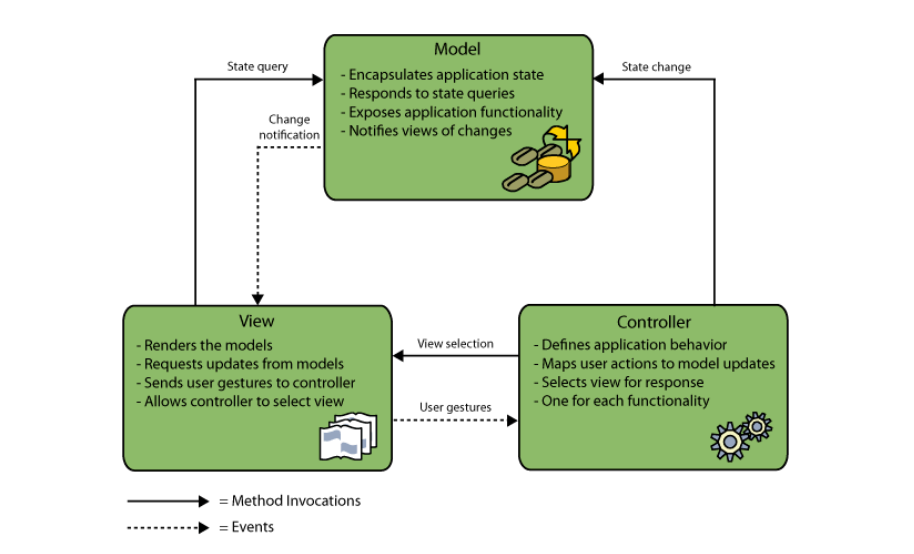
\includegraphics[scale=0.6]{Imm/mvc-archi.PNG}
\end{figure}

Nella pratica, nelle pagine HTML statiche, la view è il browser, il controller è il web server e il model sono i file html e i file di stile. Quello che succede, è che le richieste vengono inoltrare attraverso un URI, questo è uno standard attraverso il quale possiamo inviare query nella forma $urlPagina/?name=Alice\&altro=Bob$. Quello che ci viene ritornato sono dati risedenti sul web server(magari presenti in un campo hidden). \\

Nelle pagine dinamiche invece, il model è la logica di business (o logica applicativa) (ad esempio un’implementazione Java), la view è il rendering dei dati dell’applicazione (ad esempio pagine JSP) e il controller è la presentazione logica (ad esempio le servlet).

\subsection{HTML Forms}
Trasmettono le informazioni dai Web Browsers alle Web applications (URI + dati), solitamente sotto forma di elementi FORM.\\ Gli attributi che vengono considerati sono:
\begin{itemize}
   \item ACTION, che processa i dati, 
   \item METHOD che se è impostato a GET, invia i dati attraverso il l’URI, mentre se è a POST, manda i dati nel body.
   
\end{itemize}
\subsection{Servlet}
Componente Web Java-based progettato per generare contenuti dinamici. NEl caso illustrato si nota facilmente come attraverso il Browser, che ricordiamo sia la nostra view, inoltriamo delle richieste HTTP alla Servlet (Che non è il nostro WebServer, ma è una componente del server Applicativo. Pensiamo ad esempio a una JSP che si appoggia su tomcat per gestire le richieste.)
\begin{figure}[H]
    \centering
    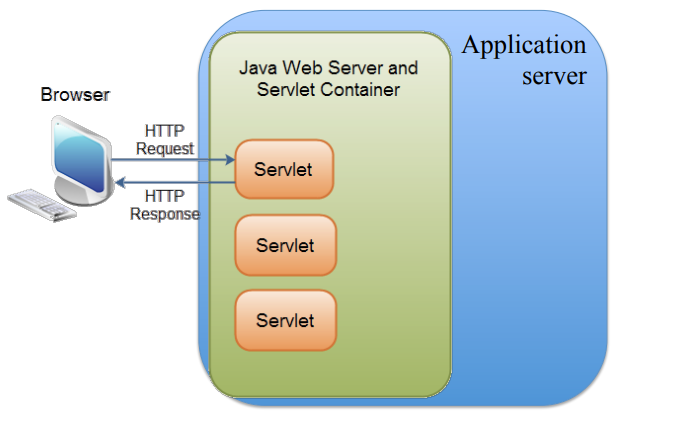
\includegraphics[scale=0.6]{Imm/jsp-servlet.PNG}
\end{figure}

\subsubsection{Ciclo di vita di una servlet} 
gestito dal container

\begin{figure}[H]
    \centering
    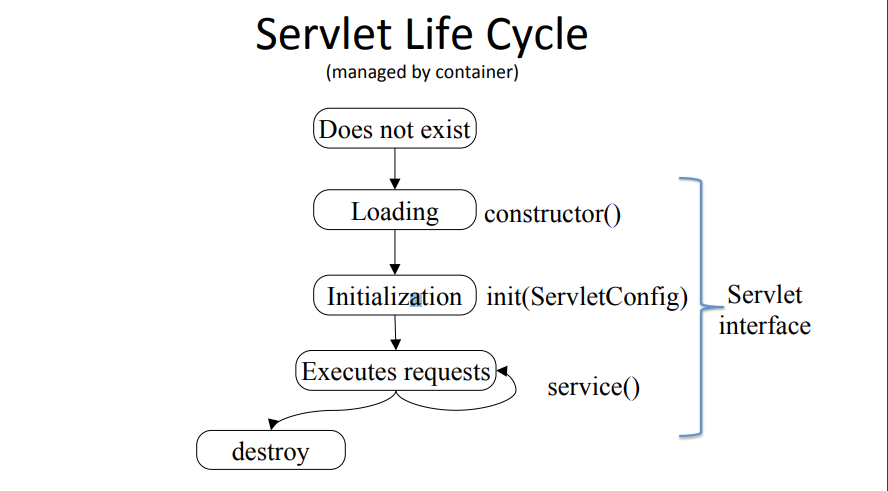
\includegraphics[scale=0.6]{Imm/servlet-life.PNG}
\end{figure}

\begin{lstlisting}
    //HttpServlet class
    abstract class HttpServlet implements Servlet
        
    //metodi aggiuntivi
    doPost(HttpServletRequest, HttpServletResponse)
    doGet(HttpServletRequest, HttpServletResponse)
\end{lstlisting}


Per gestire le richieste, si implementa \textit{HttpServletRequest} che dà un significato ai parametri della get request (dati utente inseriti in una form). Per reperire informazioni: \textit{Object user = request.getParameter("user")}\\
Il tempo di vita di un oggetto richiesto è limitato dal metodo \textit{service()} della servlet.

\subsection{Cookies}
Piccola stringa che può essere memorizzata in un client. Possono essere usati per identificare un user con una sessione web di lunga durata, per memorizzare alcuni dati interessanti sul client (nickname, id, numero di carta), per personalizzare il sito sulla base del profilo utente.\\
Il browser restituisce un set di cookies al sito e la Web applications utilizza le loro informazioni nella sua logica.

\begin{lstlisting}
    //To create cookies
    Cookie c = new Cookie('name', 'value');
    resp.addCookie(c;)
    //To get cookies
    Cookie cArray[] = req.getCookies();
\end{lstlisting}


\subsection{Session}
Una sessione è una serie di richieste associate una all’altra. Mantenere una sessione è difficile a causa della natura del protocollo HTTP.\\
Esistono diversi meccanismi per tracciare sessioni differenti: cookies, URL rewriting e hidden form fields. È il server che si occupa di gestire le sessioni.

\begin{lstlisting}
    //Getting session
    Session session = req.getSession(true);
    //Storing session infomartion in session 
    session.getAttribute(name, valueObject);
    //Retrieving information from session
    session.getAttribute(name);
\end{lstlisting}

\subsection{Sharing Data}
Ci sono diversi posti dove le servlet possono memorizzare e recuperare i dati.

\begin{table}[H]
    \centering
    \begin{tabular}{|l|l|}
        \hline
        \textbf{Place} & \textbf{Scope}                         \\ \hline
        Request        & Esecuzione del metodo service          \\ \hline
        Session        & Richieste multiple da un stesso utente \\ \hline
        ServletContext & Application-wide                       \\ \hline
    \end{tabular}
\end{table}
\textbf{Application-wide} significa che i dati devono poter essere accessibili attraveso tutta l'applicazione in modo condiviso. Stessa situazione si ha quando si usa \textit{Application Context} all'interno delle applicazioni Android.

\subsection{Threading}
Una servlet per container condivide tra multipli user e richieste, gestisce il multiThreading e presta attenzione quando accede ai dati nella sessione e nel contesto della sessione.

\subsection{JSP (Java Server Pages)}
Servono per incorporare elementi dinamici nella pagine web statiche.
Le pagine JSP sono compilate nelle servlet Java prima di essere eseguite.
(Richiesta di una pagina, generazione di una servlet da una pagina JSP, memorizzazione di una servlet per un utilizzo successivo, esecuzione di una servlet)

\begin{lstlisting}
<%=%> //JSP expression: usata per visualizzare una variabile Java
<% %> //JSP Scriplet: usata per il codice Java normale 
\end{lstlisting}

\subsubsection{Tag Libraries}
JSP supporta l’uso di librerie di tag standard e personalizzabili.
\begin{lstlisting}
<%@ taglib uri = "URIToTagLibrary" prefix="tagPrefix" %>
\end{lstlisting}

\subsection{Design Patterns}
Ci sono diversi Design Pattern, ogni pattern risolve, in lineea di massima, un determinato tipo di problema che ci si presenta.
\begin{itemize}
    \item \textbf{Controller Design}
    \begin{itemize}
        \item \textbf{Page Controller} si implementa un controller per ogni pagina.\\
         Responsabilità principali: controllare i parametri di richiesta e invoca la logica di business, selezionare la prossima vista da mostrare e preparare i dati per la presentazione.\\

        Control flow: il controllo si sposta dalla Web Server al PageController, che estrae i parametri dalla richiesta, utilizza dei business object, decide la view successiva, prepara i dati da mostrare nella view successiva e infine cede il controllo e i dati alla View.\\
        Possibili implementazioni: server page (ASP, JSP, PHP), con poca logica di controllo, o script (CGI script, servlet), con una logica di controllo significativa.\\
        È scalabile.
        \item \textbf{Front Controller} a differenza del Page controller, il Font Controller è un componente singolo che riceve le richieste da tutte le componenti della view.
        Definisce un singolo componente che gestisca tutte le richieste, eseguendo prima le operazioni comuni a tutte le richieste e poi quelle specifiche.\\
        Si divide in: 
        \begin{enumerate}
            \item \textit{Handler}: riceve le richieste dal server, esegue le operazioni generali/comuni, decide le operazioni che devono essere eseguite e delega l’esecuzione al Concrete Command.
            \item \textit{Concrete Command}: estrae i parametri dalla richiesta, invoca i metodi implementati nella logica di business, determina la view successiva e cede il controllo alla View.
        \end{enumerate}
        Il Front Controller è più complesso del Page Controller, evita che ci sia codice duplicato tra i controller, facilita la configurazione del server (solo una servlet), ha la possibilità di gestire dinamicamente nuovi comandi e è facile estendere il controller (perché ce n’è solo uno).\\
        In alcuni casi, i comandi possono essere implementati come metodi anziché come classi.\\
        È scalabile.
        \item \textbf{Intercepting Filter} 
        Utile per gestire le richieste e le risposte prima che vengano soddisfatte.
        Spesso usato con Front Controller, per aggiungere alle richieste e alle risposte funzioni aggiuntive come il logging, l’autenticazione, la conversione dei dati e l’internazionalizzazione.
        \begin{figure}[H]
            \centering
            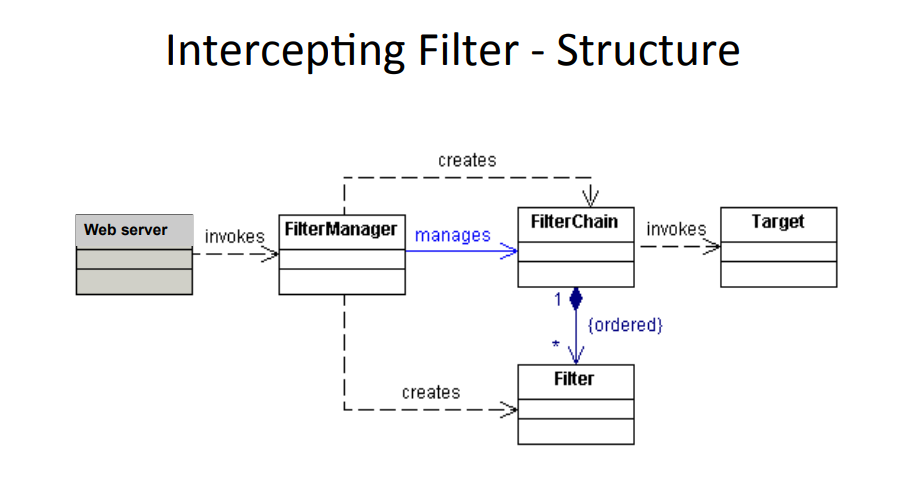
\includegraphics[scale=0.6]{Imm/if-struttura.PNG}
        \end{figure}
        Il Web Server solitamente fornisce il FilterManager e il FilterChain; quindi c’è solo bisogno di implementare e dichiarare i Filtri.
        \begin{figure}[H]
            \centering
            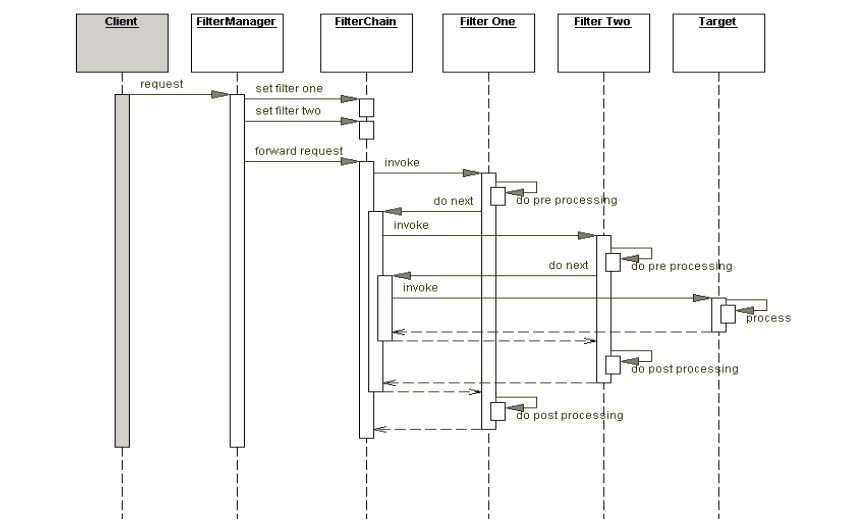
\includegraphics[scale=0.6]{Imm/if-behave.PNG}
            \caption{Qui possiamo notare in un diagramma a sequenza le varie interazioni che si hanno a Partire dal Client fino al raggiungimento del Target}
        \end{figure}
        \item \textbf{Application Controller}: Quando cresce la complessità del flow, il management del flow potrebbe essere concentrato in una classe.
         \begin{figure}[H]
            \centering
            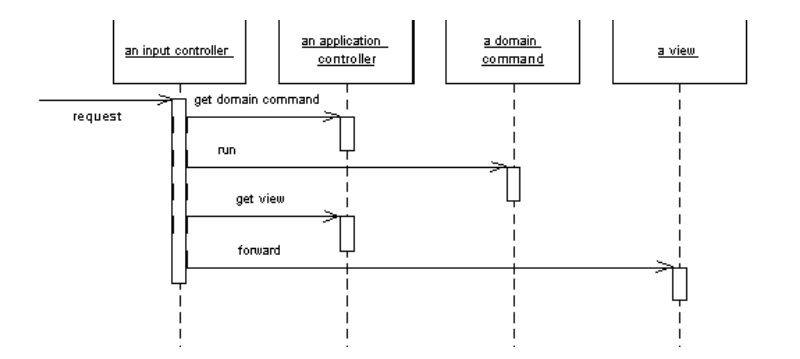
\includegraphics[scale=0.6]{Imm/ac-diagram.PNG}
            \caption{Questa tipologia di approccio viene tipicamente utilizzata dal Page Controller o dal Front Controller}
        \end{figure}
    \end{itemize}
    \item \textit{View Design}, una seconda categoria di pattern, che riguarda più la costruzione delle pagine invece che concentrarsi sul controllo di dati.
    \begin{itemize}
        \item \textbf{ Template View}: La parte di rendering viene ottenuta definendo parte di contenuto statico e parte di contenuto dinamico il cui effettivo valore dipende dal modello e dal suo stato. \\
        Utilizza le classi Helper create dal Controller, per facilitare la costruzione della pagina: la pagina non fa diretto accesso al modello ma fanno riferimento all’Helper che a sua volta fa riferimento al Model. L’Helper prepara dei dati ad hoc per la parte di presentazione.\\
        Il Block-helper genera codice HTML dalle pagine di template che includono chiamate al modello. Genera i dati di dominio, separa la View dall’implementazione logica ed è creato da un controller e acceduto da una View.
        \item \textbf{Transformation View}  Non si ha una pagina template con parti costanti e parti dinamiche ma la pagina viene creata interamente in modo dinamico a partire dai dati che devono essere presentati. Il componente responsabile per la costruzione di questa pagina è il Transformer.\\
        Trasforma le entità di dominio in HTML. Una tipica implementazione del modello è quella in cui ogni classe di dominio implementa la funzione toXML(). Una tipica implementazione del Transformer usa XSLT (eXtensible Style), un linguaggio per le trasformazioni.\\
        Transformation View si focalizza sull’entità che dev’essere trasformata piuttosto che sulla pagina di output (Template View).\\
        È difficile da includere l’implementazione logica nella View; è però facile da testate (controllando lo stream che si genera dopo la trasformazione XSLT) ed è facile da applicare a dati XML.\\
        WYSIWYG è più intuitivo e facile da gestire.
        \item \textbf{Two-Steps View} Genera la pagina HTML in due steps: genera una pagina logica e renderizza la pagina.\\
        Appare facile da modificare perché il rendering non interferisce con la struttura dell’informazione che dev’essere visualizzata sulla pagina.
        L’implementazione consiste nella sequenza di due trasformazioni XSLT: costruire la pagina logica e renderizzare la pagina.
        La Templete View ha dei tag personalizzabili.
        Quindi la pagina HTML è la pagina logica e i tag personalizzabili effettuano il rendering.
    \end{itemize}
\end{itemize}
\subsection{Struts 2}
Struts è un framework open source per lo sviluppo di applicazioni web su piattaforma Java EE, nella versione 2 garantisce un'ulteriore riduzione dei tempi di sviluppo grazie ad un'ulteriore semplificazione della logica e della corrispettiva implementazione del framework. Non è altro che un insieme di classi ed interfacce che costituiscono l'infrastruttura per costruire Web Application Java EE(Enterprise Edition) conformi al design pattern MVC.\\
In questo tipo di framework possiamo definire, invece che implementare, il flow delle azioni che devono essere svolte. Quindi per l'implementazione di una determinata operazione, usando Struts2, ci sere eseguire: l'implementazione della view, delle azioni, e la \textbf{definizione}, e non implementazione, di un flow.

\subsection{Spring MVC}
Framework: implementazione integrata di pattern design multipli.
Il flow può essere definito anziché implementato.
L’implementazione di un’operazione tipicamente richiede l’implementazione della View e dell’azione e la definizione del flow.
\section{Object Relational Mapping (ORM)}
Come sappiamo non si ha una relazione diretta tra OOP(Object Oriented Programming) e modello relazionale e per questo si usa l'\textbf{Object Relational Mapping (\textit{ORM})} quando si lavora con la OOP ma con dati persistenti in un database (con le classi che vanno mappate nelle entità e viceversa). Esistono dei framework che utilizzano implementano questa tecnica.\\
Quello che si cerca è di avere una costruzione che sia quanto più possibile trasparente, rispetto alla parte di persistenza e memorizzazione dei dati, e che ci permetta di scrivere il codice in modo coerente, riferendoci unicamente al modello Object Oriented. Molti dei concetti si applicano ad altri framework, che magari non mirano al solo Object Oriented.\\
La soluzione al ORM (quindi alla tecnica di relazionamento), dal punto di vista architetturale, prevede un Client che utilizza un Model e dati che devono rimanere persistenti su una Resource. Il problema risulta il far comunicare Client e Resource. La soluzione è data dall'inserimento di un API Gateway che ha il compito di eseguire la traduzione bilaterale della comunicazione tra i due elementi.\\
Concretamente diremo che si sfrutta un \textit{API gateway} tra il client e le risorse dati (il database in questo caso) che incapsula l'accesso a una risorsa esterna con una classe e traduce le richieste di accesso alla risorsa esterna in chiamate all'API. Con questo approccio si nasconde l'accesso alle risorse (rendendone anche facile la modifica) e la complessità delle API.
\subsection{database Gateway}
Si hanno tipicamente 4 pattern per il \textbf{database gateway}:
\begin{itemize}
    \item \textbf{Table Data Gateway}, che prevede un oggetto che funge da gateway per una determinata tabella del database. Dispone di un'interfaccia semplice, solitamente costituita da: diversi metodi di ricerca per ottenere i dati da database, metodi di update, insert e delete. Ogni metodo mappa i parametri di input in una chiamata SQL e esegue l'SQL su una connessione al database. Il Table Data Gateway è solitamente privo di stato (stateless), poiché il suo ruolo è quello di portare i dati avanti e indietro. Un problema del TDG è che anche una semplice query di ricerca tramite ID restituirà più elementi, invece che uno. In ambienti in cui puoi restituire più elementi, puoi utilizzare quelli per una singola riga, ma molti liuguaggi forniscono un solo valore di ritorno e molte query restituiscono più righe. Risulta comodo nel paradigma procedurale ma meno in quello OOP in quanto i metodi ritornano dati row e non oggetti.
    \item \textbf{Row Data Gateway}, prevede un oggetto che funge da gateway per un singolo record all'interno del data source. Prevede quindi un oggetto per record, comportando che si possono avere più copie di oggetti persistenti in memoria, avendo una classe gateway che funge da alter-ego del database che viene chiamata dalla classe coi metodi \textit{finder} (che però potrebbero essere implementati direttamente nella classe gateway).
    \item \textbf{Active Record}, che prevede un oggetto per record
    \item \textbf{Data Mapper}, che prevede un layer applicativo dedicato all'ORM
\end{itemize}
\subsubsection{Active record}
Questo pattern è una versione ottimizzata del \textit{row data gateway}.\\ Considerate le classi che implementano i dati che devono essere persistenti si arricchiscono le classi con metodi per permettere l'interazione col database. Un \textbf{active record} include quindi:
\begin{itemize}
    \item la business logic
    \item il mapping logico al database, avendo come metodi statici i \textit{metodi finder} (quelli spiegati nel TDG, invocabili avendo accesso alla classe) che comunque restituiscono risultati già nel dominio OOP (oggetti o collezioni di oggetti). Si hanno inoltre metodi non statici i \textit{metodi gateway} (per lavorare con le istanze)
\end{itemize}
Tra i metodi abbiamo quindi:
\begin{itemize}
    \item \textbf{metodo load}, che crea un'istanza a partire dai risultati di una query SQL. Potrebbe essere necessario creare altri oggetti con accesso a più
    tabelle nel casi di reference
    \item \textbf{costruttore}, per creare nuove istanze che saranno poi rese persistenti invocando metodi appositi
    \item \textbf{metodi finder}, statici, che incapsulano la query SQL e ritornano una collezione di oggetti
    \item \textbf{metodi write}, tra cui si hanno:
    \begin{itemize}
        \item \textbf{update}, per aggiornare un record a seconda dei valori degli attributi 
        \item \textbf{insert}, per aggiungere un record a seconda dei valori degli attributi 
        \item \textbf{delete}, per cancellare il record corrispondente all'oggetto in analisi
    \end{itemize}
    serve sincronizzazione tra oggetto in memoria ed entità nel database. Per farlo si ha un attributo identificatore nella classe che compare anche nel record e che serve per trovare il record corrispondente ad un oggetto
    \item \textbf{metodi getter e setter}, che a seconda del caso devono essere subito sincronizzati con il database
    \item \textbf{metodo business}
\end{itemize}
Si nota quindi che è una semplice implementazione ORM senza separazione tra business logic e meccanismo di persistenza, tendendo a forzare una corrispondenza ``uno a uno'' tra oggetti della OOP e istanze nell'ER (anche se questo vale per molti pattern).
\subsubsection{Data mapper}
Con il pattern \textbf{data mapper} invece si ha un layer software indipendente dedicato alla persistenza e all'ORM, in modo che la logica di dominio non conosca la struttura del database e nemmeno le query SQL. Si usano quindi interfacce per consentire l'accesso ai mapper indipendentemente dalla loro implementazione.
\begin{figure}[H]
    \centering
    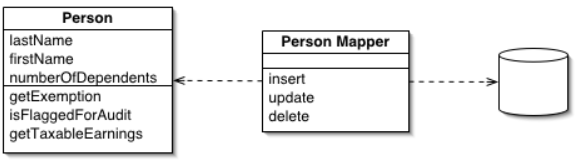
\includegraphics[scale = 0.6]{Imm/databaseMapperSketch.png}
    \caption{Esempio di UML di data mapper, dove si nota la separazione della classe dai metodi dedicati alla persistenza (nel mapper).}
\end{figure}
Framework moderni implementano questo tipo di pattern (che offre la parte di mapping senza doverli implementare ,a solo configurare). 
\subsection{Ulteriori pattern ORM}
L'aspetto del mapping è solamente una piccola parte del intero procedimento, questo perché si hanno altri problemi da dover risolvere e in generale, assocciati ai problemi, si hanno dei pattern di comportamento per risolverli. Possiamo fare una distinzione dei pattern in Comportamentali e Strutturali.
\begin{itemize}
    \item \textbf{Comportamentali}, in questa sezione abbiamo i pattern: unit of work, identity map e lazy load.
    \item \textbf{Strutturali}, abbiamo invece: value holder, identify field, embedded value e LOB
\end{itemize} 
\subsubsection{Unit of work}
In questo caso si approfondiscono le operazioni ACID cercando di capire quando sincronizzare le informazioni \textit{in memory} con il database. Questo aspetto è importante introducendo il concetto di \textbf{business transaction} per operazioni, che dal punto di vista dell'utente, devono essere eseguite con semantica di tipo \textit{all or nothing} dove o si accettano tutte le operazioni richieste o nessuna (si pensi ad esempio alla prenotazione di un biglietto). Le business transaction vanno quindi mappate nelle \textbf{system transaction} fatte dal sistema sul database. Si hanno diverse soluzioni:
\begin{itemize}
    \item \textit{aggiornare il database ogni volta che si ha una modifica in memory (slide 25)}. In pratica business transaction e system transaction coincidono ogni volta, dall'apertura alla chiusura oppure ogni volta che l'utente modifica qualcosa si effettua una system transaction. La prima soluzione è poco pratica a causa di transazioni molto lunghe (\textit{long-lasting database transactions}) in quanto un perfetto isolamento implica gestire/servire una sola query alla volta mentre un isolamento imperfetto implica che si hanno transazioni che leggono dati non definitivi, comportando inconsistenze. L'utente può aprire la transazione e restarci minuti, questo comporta anche un peggioramento delle performance del database perché blocco altre operazioni.
    \item \textit{Aggioranre il database ad ogni operazione (slide 26)}. Invece di aggiornare il database una volta sola per intera operazione,quindi da \textbf{begin} a \textbf{commit}, eseguo un aggiornamento per ogni operazione eseguita. Con il secondo caso si rischia di non poter implementare l'atomicità delle transazioni di business, che se in un certo momento fallisce non impedisce alle vecchie modifiche di essere già scritte, rompendo la \textit{all or nothing}, avendo molte difficoltà nel fare gli \textit{undo}
    \item \textit{tracciare le operazioni (nella transazione di business) e attuare tutte le modifiche in una singola transazione di sistema (slide 27)}. Tutte le operazioni sul sistema si eseguono alla fine. Il software tiene memoria di tutte le operazioni svolte dall'utente, e solamente alla fine viene avvita una transazione coin il database, in questo modo vengono eseguite tutte le notifiche al database. 
\end{itemize}
La unit of work quindi traccia ogni cambiamento (coi metodi \textit{register}) e lo attuta in una singola system transaction finale (con il \textit{commit}). Per fare questo incapsula ogni update/insert/delete, mantenendo l'integrità del database ed evitando deadlock.\\ 
A proposito di locking si ha che due business transaction possono essere attive nello stesso momento e bisogna capire come devono lavorare sul database. In questo caso si hanno due strategie:
\begin{itemize}
    \item \textbf{optimistic locking}, usato quando si hanno poche probabilità di generare conflitti, avendo diversi utenti che lavorano spesso su dati differenti, e si bassa su un numero che identifica la versione degli oggetti registrati. L'ottimismo di non avere più persone che lavorano sugli stessi dati, si traduce in record che non vengono bloccati, quindi le business transaction possono quindi interferire accedendo e modificando i record ma si sfrutta, un elemento salvato nel database, ovvero il numero di versione per tenere traccia delle modifiche. Se una transazione vede che il numero di versione di un record è incrementato significa che qualcun altro ha fatto una modifica dopo che la business transaction ha caricato l'oggetto, c'è quindi stato una modifica concorrente. In  tal caso si ricarica il record tramite un rollback e iniziamo da capo.
    Esempio di diagramma di sequenza:
    \begin{figure}[H]
        \centering
        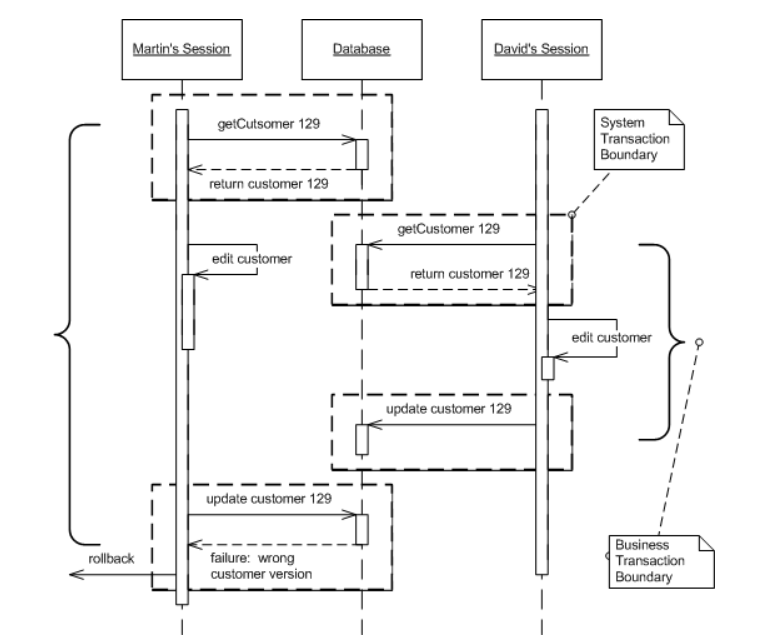
\includegraphics[scale = 0.5]{Imm/OptimisticSketch.png}
    \end{figure}
    \item \textbf{pessimistic locking}, usato quando hanno alte probabilità di generare conflitti. Gli oggetti sono bloccati non appena vengono usati riducendo la concorrenza. Non si permette quindi alle transazioni di lavorare concorrentemente riducendo però le prestazioni del sistema ma aumentando la sicurezza. Esempio di diagramma di sequenza:
    \begin{figure}[H]
        \centering
        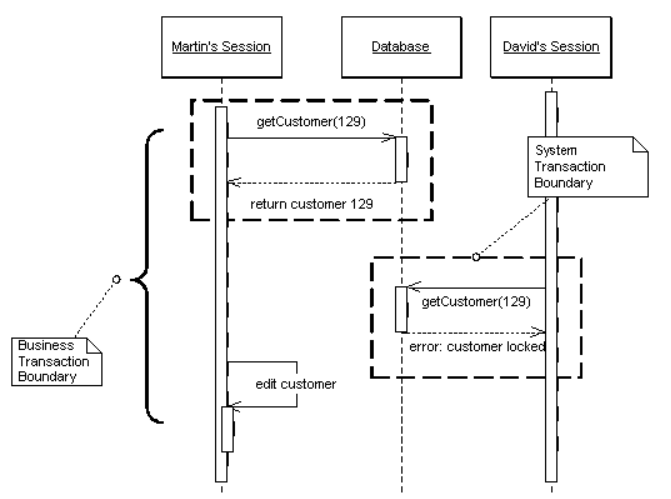
\includegraphics[scale = 0.5]{Imm/PessimisticSketch.png}
    \end{figure}
\end{itemize}
Poi, per avvisare la unit of work che un'operazione  deve essere eseguita, si hanno due pattern:
\begin{itemize}
    \item \textbf{caller registration}, dove chi modifica l'entità lo notifica direttamente alla unit of work. Questa soluzione è rischiosa in quanto il programmatore potrebbe dimenticarsi di notificare la UoW, ma permette maggior flessibilità, permettendo di decidere dinamicamente se i cambiamenti devono riflettersi sullo storage persistente. 
    \item \textbf{object registration}, dove è l'entità modificata a notificare la unit of work, che però deve obbligatoriamente avere accesso globale. Ogni cambiamento viene comunque notificato. Solitamente si usa questa soluzione ma nella variante in cui le classi persistenti non includono il codice per la notifica ma tramite una strumentazione automatica e trasparente offerta dai framework.
\end{itemize}
\subsubsection{Identity map}
In questo caso si studia il load di un'istanza direttamente a partire dal database. Se un certo record viene richiesto due volte si generano due oggetti uguali (esempio prima chiedo lo \textit{user1} e poi tutti gli \textit{user} (che ipotizziamo siano \textit{user1 \textnormal{e} user2}), avendo alla fine due copie istanziate di \textit{user1}). In pratica uno stesso oggetto può essere caricato più volte, o da azioni differenti dello stesso utente (rischiando inconsistenze, se una istanza viene modificata, oltre ad avere ridondanza di dati) o da utenti diversi (in questo spesso è intenzionale).\\ \textbf{Identity map} è quindi un oggetto con la responsabilità di identificare gli oggetti caricati in una sessione, funzionando come una sorta di cache, controllando l'eventuale presenza dell'oggetto ``in cache'' (anche se non si ha una vera cache) prima di caricarne uno nuovo (se già presente si ritorna un riferimento all'oggetto). Identity map quindi mantiene i riferimenti agli oggetti tramite un sistema chiave-valore.\\
\begin{figure}[H]
        \centering
        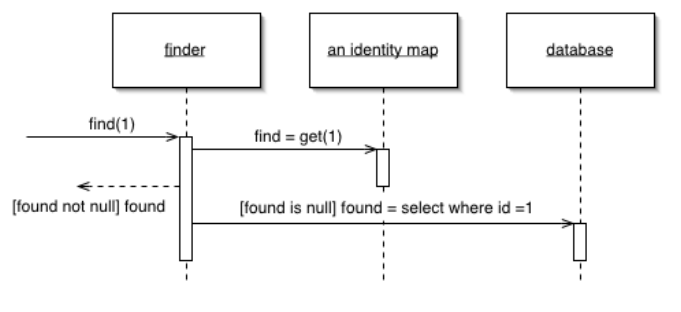
\includegraphics[scale = 0.5]{Imm/i-map.PNG}
    \end{figure}
Generalmente la chiave della mappa è quella primaria del database. Si hanno delle identity map in base al contesto di utilizzo:
\begin{itemize}
  \item una per applicazione, solo se le chiavi di entità differenti sono disgiunte
  \item una per classe, è l'opzione di default
  \item una per tabella, generalmente meglio se una per classe
\end{itemize}
La mappa è sempre accessibile.\\
\subsubsection{Lazy load}
A volte è necessario avere solo una parte di un oggetto per eseguire una certa operazione anche perché alcuni attributi (collection, bitmaps, grafi) possono essere particolarmente pesanti. Si parla quindi di efficienza.\\ 
Si procede quindi con il pattern \textbf{lazy load} che non carica i valori per alcuni attributi delle classi e caricarle solamente \textit{on-demand}, ovvero solamente se l'applicazione cerca di accedervi.\\ \textit{si aggiunge: } \textbf{Lazy load} quando crea oggetti inizializza solo alcuni attributi, evitando spesso quelli più pesanti e quelli che meno si usano, lasciando comunque possibilità si caricare in seguito ulteriori attributi non ancora inizializzati se ce ne fosse necessità, in modo \textit{on-demand}, tramite i \textit{finder}.\\ 

\subsubsection{Value holder}
Con questa tecnica si usa un oggetto, il \textbf{value holder}, come uno storage intermediario per un attributo. Anche in questo caso si ha un'inizializzazione lazy, infatti l'oggetto usato in questione, in base al caso d'uso potrebbe essere istanziato con diverse strategie di load. Si separa la logica di dominio da quella lazy di loading.\\

\subsubsection{Identify field}
Normalmente si hanno: l'identità in memory rappresentata dalla reference dell'oggetto e l'identità nel database rappresentata dalla chiave primaria. Per le quali si ha bisogno di accoppiare/sincronizzare le due identità per la consistenza dei dati.\\ 
La soluzione è usare l'\textbf{identity field} ovvero un nuovo attributo (campo) nell'oggetto il cui valore diventa la chiave primaria (solitamente chiamato \texttt{id}, di tipo \texttt{long}). Non si usano i normali attributi/identificatori della classe perché potrebbero modificare nel tempo di sviluppo del programma.\\
Si hanno infatti due tipi di chiave:
\begin{itemize}
  \item una chiave derivata da attributi dell'oggetto (che sono usati anche dall'applicazione, ad esempio la matricola). Si ha comunque rischio di duplicazione, possibile assenza di valore e cambiamenti sulla logica di dominio che impattano su quella di persistenza
  \item chiavi dedicate, sia semplici (un solo attributi) che composte (di più attributi), avendo una chiave per tabella e una per database. Nella pratica spesso hanno tipo \texttt{long} che ben supporta il check di uguaglianza (\texttt{==}) e la generazione di nuove chiavi
\end{itemize}
Si hanno varie strategie per la generazione delle chiavi:
\begin{itemize}
  \item direttamente dal database (con sequenze o id delle colonne)
  \item tramite \textit{GUID}, ovvero Globally Unique IDentifier, tramite opportuni software e libreria
  \item dall'applicazione, principalmente in due modi:
  \begin{itemize}
    \item \textit{table scan}, usando una query SQL per determinare il valore della prossima chiave
    \item \textit{key table}, usando tabelle speciali con il nome delle altre tabelle e il valore successivo della chiave
  \end{itemize}
\end{itemize}
I moderni framework ORM supportano i vari design pattern appena discussi e quelli mancanti, relativi a chiavi esterne, cascading, ereditarietà. \\ In ogni caso i pattern appena discussi sono tutti supportati dai moderni framework ORM.

\subsubsection{Embedded value}
Con questo pattern si hanno semplici oggetti, senza un chiaro concetto di identità, che possono essere inclusi in oggetti che fungono da alter-ego delle tabelle anziché creare tabelle dedicate.

\subsubsection{LOB}
Vediamo ora il pattern \textbf{Serialized Large Object (\textit{LOB})} che consiste in un grafo di oggetti memorizzati del database tramite serializzazione.\\
Questo pattern è comodo finché il LOB può essere gestito come un \textit{embedded value} ma si hanno problemi se vengono usati attributi serializzati nelle query o se il grafo ha dipendenze con oggetti non serializzati.\\ 
Si ha \textbf{Binary LOB (\textit{BLOB})}, semplice da implementare (ad esempio con \textit{Java serialization}) e compatto. Purtroppo si ha che un BLOB non è stampabile e si ha che il database deve supportare tipi binari. Crea anche problemi con il versioning delle classi.\\ 
Si ha anche \textbf{Character BLOB (CLOB)}, ad esempio tramite \textit{XML}, che però richiede librerie per il parsing e non è compatto, anche se stampabile e supportato generalmente dai database

\section{JPA 2.0}
Noi troviamo all'interno dei framework i metodi e i vari meccanismi implementati, noi dobbiamo fruire di quest'ultimi in modo dichiarativo, ovvero dobbiamo solamente andare a dire come quel meccanismo/pattern deve comportasi.
Le \textbf{Java Persistence API (\textit{JPA})}, sono un framework per il linguaggio di programmazione Java che si occupa della gestione della persistenza dei dati di un database MS relazionale nelle applicazioni.\\ 
Si ha quindi un grande set di pattern già implementati che usiamo in modo dichiarativo specificando il mapping tra enità di dominio e database. Si hanno varie implementazioni di JPA con ORM (tramite annotations e services, per comandare operazioni di persistenza), tra cui \textit{Hibernate}.\\

Una JPA Application è una normale applicazione Java dove abbiamo un insieme di classi, che implementano la business logic, e tra queste si identificano le \textit{Entity Class} (classi contenente i dati che vengono mappati sul database). Oltre a queste classi, che definiamo essere sincronizzate con il database, abbiamo anche che le nostre classi interagiscono con un servizio, il \textit{Entity manager}. Entity manager è il servizio che implementa la maggior parte dei design pattern per ORM mapping e al quale noi chiediamo di fare delle operazioni sui oggetti della classe stessa. Volendo il database può essere generato automaticamente dalle Entity Class o viceversa.

\subsection{Entity Manager}
Entity class che prendono anche il nome di \textbf{Plain Old Java Objects (\textit{POJO})}, inoltre gli oggetti che vengono creati tramite il \texttt{new} e che sono oggetti regolari fino a che non interagiscono con l'\textbf{Entity Manager} (sono normali classi con annotazioni).\\ 
Un'entità in memoria può essere in due stati:
\begin{itemize}
    \item \textbf{managed/attached}, se l'entità è sotto gestione dell'Entity Manager. Tramite tale interazione con l'Entity Manager le entità sono memorizzate nell'\textit{identity map} ed eventuali cambiamenti sono tracciati dalla \textit{unit of work}. Implementando la unit of work, può essere comandato per essere scaricare sul databse, in determinati momenti ben precisi, tutte le modifiche che sono state accumulate. D'altro canto create/remove sono responsabilità dello sviluppatore mentre le update sono rilevate automaticamente dall'Entity Manager.
    \item \textbf{unmanaged/detached}, se l'entità non è sotto gestione dell'Entity Manager, che non sa che esiste quell'entità
\end{itemize}
Posso spostare esplicitamente un oggetto da uno stato all'altro in quanto può essere utile avere oggetti unmanaged, spesso in caso di applicazioni distrubuite durante l'invio ad un altro nodo (diciamo che sono situazioni obbligate dalla pratica). Normalmente un oggetto managed rimane tale.
Si ha quindi uno schema del tipo:
\begin{figure}[H]
    \centering
    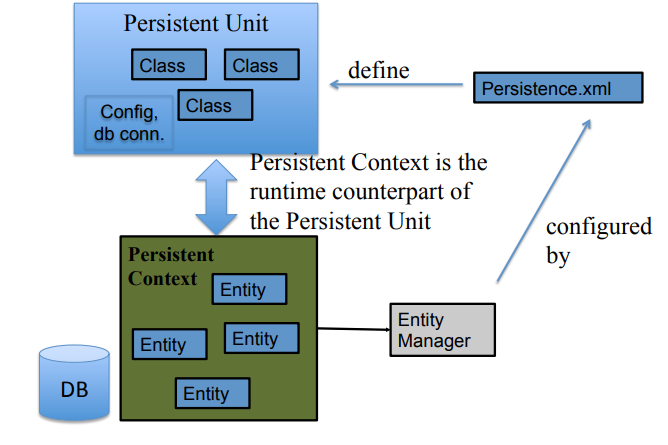
\includegraphics[scale = 0.57]{Imm/entity-manager.PNG}
\end{figure}
Nello schema si ha in alto la parte di configurazione e in basso quella di runtime. Le classi sono divise in varie \textbf{persistent unit}, ciascuna che può lavorare con un database diverso. \\ 
L'Entity Manager, che è servizio runtime con cui l'applicazione interagisce, legge il suo \textit{persistence.xml} e solamente ora sa come devono essere gestite le entità e su quale database deve mantenere la persistenza.\\

Il file \texttt{persistence.xml} è contenuto nella cartella \texttt{META-INF} del progetto e gestisce tutte le varie configurazioni. Sono indicate nel file le classi della \textit{persistent unit}: ovvero tutte le classi di entità nel progetto java (con il tag \texttt{<class>}) o contenute in un jar (con il tag \texttt{<jar-file>}).\\

In merito al mapping tra classi e database si ha che esso è definito tramite annotazioni nelle classi e all'interno dei file XML intenti a ricoprire il l'orm-mapping. I fil XML devono essere specificati all'interno del \texttt{persistence.xml} tramite il tag \texttt{<mapping-file>}.\\ 
\textbf{Nelle query si usano comunque i nomi degli oggetti}.\\
\textit{Fa un esempio di JPA completo in JAVA, seguito, ma niente di $>>$}

\subsection{Mapping}
Abbiamo diversi tipologie di mapping. Ricordiamo che indichiamo con \textit{@Entity} la nostra POJO.
\begin{itemize}
    \item \textbf{Mapping to Tables}, si identifica la classe in questione, ovvero la nostra Entity, e la si mappa con la tabella del database. Per farlo si aggiunge la notazione \textit{@Table(name="NomeTabellaDb")}. In seguito ogni attributo della classe può essere mappato come colonna della tabella attraverso \textit{@Column(name="NomeColonna")}
    \item \textbf{Simple Primary Key}, si riferisce al metodo di generazione di una chiave primaria (solitamente l'id, che spesso si trova essere di tipo Long) semplice. Alla entity va specificato che verrà utilizzato un sequenza generatrice dipendente dal DB (\textit{@SequenceGenerator}), e in seguito si specifica che la generazione è obbligatoria (\textit{@GeneratedValue}) indicando in base a quale criterio eseguire la generazione (strategy=GenerationType.Strategia, generator=“Criterio”).  
    \item \textbf{Una entità due tabelle}, come visto nel caso di \textit{Mapping to Tables}, avevamo che una tabella veniva rappresentata come singola Entity, in questo caso invece la Entity è rappresentata da due tabelle, e due tabelle sono mappate da una sola Entity. Per mappare una seconda tabella nella Entity usiamo \textit{@SecondaryTable(name=“Tabella2”, pkJoinColumns={@PrimaryKeyJoinColum(name=“PK2Tab”)})}
\end{itemize}

Possiamo anche andare a dichiarare che un determinato attributo di una certa Entity è incorporabile. Ci serve solamente specificare che la classe da incorporare sia annotata con \textit{@Embeddable}, e nella Entity usare la \textit{@Embedded} notazione per poi andare a utilizzarla.\\

Possiamo inoltre aggiungere che le chiavi primarie utilizzano la notazione \textit{Long} per via dell'efficienza che comporta avere valori di tipo Long nei confronti di uguaglianza. \\

\subsection{Refernce tra Entity diverse}
Segue lo stesso concetto del linguaggio SQL:
\begin{itemize} 
    \item \textit{One-to-One} monodirezionale, la chiave primaria \textit{a} della tabella \textit{A} è anche chiave esterna referenziata da una colonna \textit{b} della tabella \textit{B}. Ricordiamo che ogni tabella è rappresentata da una singola Entity nel JPA.
    \item \textit{One-to-One} bidirezionale, segue lo stesso principio della mono, con la particolarità che possiamo tenere traccia attraverso \textit{mappedBy} per capire quale Entity ha eseguito il mapping. Quindi per entrambe le Entity abbiamo un reference per la Entity in relazione. 
    \item \textit{One-to-Many}, vengono create delle collezioni di dati. I dati vengono ritornati dalle operazioni di Join tra le tabelle in relazione.\textit{Una Entity può avere collegate più record di un attributo di una seconda Entity}
    \item \textit{One-to-Many} bidirezionale, vengono sempre create delle collezioni di dati, da una parte abbiamo una relazione \textit{Many-to-One}, nell'altra entity invece abbiamo una \textit{One-to-many} per la collezione dati di cui si parlava prima. 
    \item \textit{Many-to-One}, usa il metodo inverso utilizzato dalla One-to-Many. 
    \item \textit{Many-to-Many}
\end{itemize}

\subsection{Mapping Hierachies}
Nella OOP posso avere gerarchie tra gli oggetti ed ereditarietà ma questi concetti non si hanno nei database e quindi serve un mapping dedicato per eseguire query che sfruttano le gerarchie. Il mapping deve essere esplicitamente specificata.\\ Si hanno tre strategie per il mapping (\textbf{su slide esempi delle varie annotazioni per Java}):
\begin{enumerate}
      \item \textbf{single table}, che prevede una tabella per ogni classe in rapporto di gerarchia tra loro. Si ha quindi una colonna che deve rappresentare il tipo di oggetto (per distinguere le varie classi) di tipo stringa. È un metodo facile da implementare e veloce ma obbliga ad avere tabelle che possono contenere valori NULL (una classe derivata ha attributi in più di quella orinale e diversi da un'altra classe derivata dalla stessa classe originale etc$\ldots$). Si ha comunque uno spreco di risorse.
      \item \textbf{one table per concrete class}, dove ogni classe (sia padre che figli) hanno una tavella associata con un campo per ogni attributo (per le figlie anche quelli ereditati). Tutti gli attributi di una classe sono quindi in una singola tabella dedicata. Si ha un maggior controllo dei vincoli e un mapping ancora semplice ma è difficile da gestire con l'Entity Manager e il databaseMS deve supportare la \textit{SQL UNION}
      \item \textbf{one table per subclass} dove si ha una classe per tabella ma senza ricopia degli attributi per le classi figlie (che sono caratterizzate solo dall'id e dagli attributi extra rispetto alla classe padre). Si ha quindi un mapping ``uno a uno''. Questa strategia supporta i vincoli tabellari e non richiede la \textit{SQL UNION} ma si ha un istanza ``splittata'' su più tabelle ed è generalmente una soluzione lenta in esecuzione (dovendo eseguire i \textit{join})
\end{enumerate}
\section{Enterprise Application}
\textbf{Sviluppo per componenti}: sviluppo che permette di creare unità (componenti) di cui si può fare il deployment in modo indipendente dagli altri componenti e quindi che non hanno dipendenze statiche ma che possono essere soddisfatte a runtime nell'ambiente di esecuzione.\\

\textbf{Decoupling}: rendere indipendenti le componenti di cui si deve fare il deployment anche a runtime, per poter svolgere una funzionalità, una componente/un servizio deve interagire con un altro. Non si parla della dipendenza funzionale, che rimane; ma non ci saranno dipendenze che ostacolano il deployment (non saranno dipendenze statiche ma a runtime).\\

Opzioni per gestire dinamicamente le dipendenze:
\begin{itemize}
    \item \textit{Inversion of Control} o \textit{Dependency Injection}: i campi che memorizzano dei riferimenti ad altri componenti vengono popolati automaticamente da una componente esterna.\\
    
    L’idea è quella di introdurre un elemento esterno (l’assembler) che ha la responsabilità di creare/individuare il componente che deve essere utilizzato e iniettare la dipendenza nella classe che ne ha bisogno. Il campo viene popolato senza che la classe al cui il campo appartiene lo chieda. \\
    
    Quando la dipendenza viene iniettata? Nella maggior parte dei casi, quando l’oggetto viene creato.\\
     
    Come fare injection? Utilizzando il costruttore (Constructor Injection) mediante un suo parametro, usando un setter/field (Setter/Finder Injection) o usando un metodo dell’apposita interfaccia (Interface Injector), ma non è una strategia molto utilizzata.\\
    
    Come programmare l’assembler? L’assembler normalmente è già implementato nei framework, altrimenti andrebbe configurato secondo i file di configurazione o le annotazioni delle classi con le dipendenze da iniettare.
    \begin{figure}[H]
        \centering
        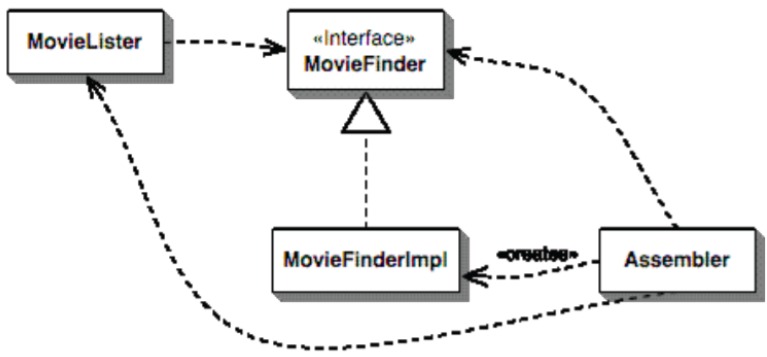
\includegraphics[scale=0.4]{Imm/inversion_control.png}
    \end{figure}
    
    \item \textit{Service Locator} o \textit{Dependency Lookup}: la classe che ha bisogno di popolare un campo con un riferimento chiede esplicitamente al Service Locator il valore di riferimento.\\
    
    L’idea è quella di avere un registro, il Service Locator, che conosce qual è l’implementazione che dev’essere usata di volta in volta. La classe che deve soddisfare la dipendenza fa un accesso al Service Locator, chiedendo che venga ritornato un riferimento al componente che dev’essere utilizzato. Quindi qualcuno popola il Service Locator, tipicamente un Assembler che crea le componenti e le aggiunge al Service Locator, specificando quali componenti esistono e che interfaccia implementano.\\
    
    Nella sua accezione più semplice, il Service Locator è un singleton che memorizza delle coppie chiave-valore, dove il valore è il riferimento alla componente che può essere utilizzata e la chiave può essere l’interfaccia che il componente implementa.\\
    
    All’interno delle classi, per poter interrogare il Service Locator, serve un riferimento al servizio di Service Locator che può essere settato attraverso dependency injection (quindi attraverso un’annotazione) o più trasparentemente alcuni framework permettono di assegnare dei nomi ai componenti (degli identificatori) e poi se un altro componente necessita di un reference a quei componenti si può utilizzare una notazione che ne specifica il nome.
    \begin{figure}[H]
        \centering
        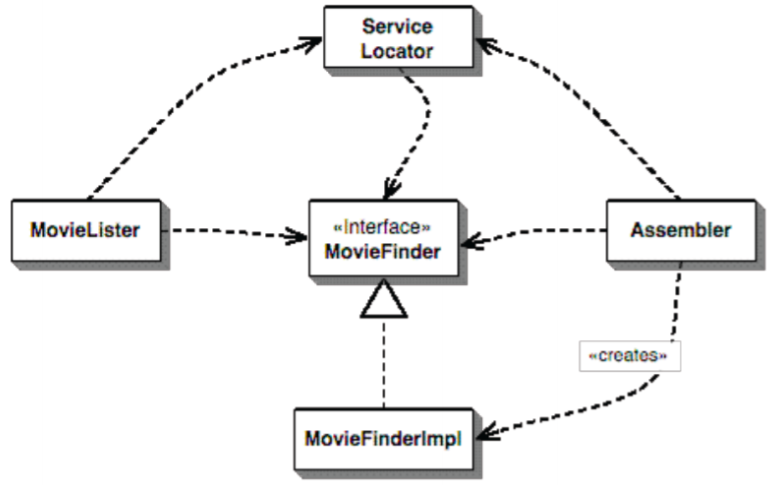
\includegraphics[scale=0.4]{Imm/service_locator.png}
    \end{figure}
\end{itemize}

\subsection{Enterprise Java Beans}
EJB 3.0 è un modello di sviluppo per componenti Java, che è uno standard. Ci sono tanti framework che implementano lo standard EJB come Glassfish, JBoss e altri.\\

Nelle applicazioni EJB ci sono componenti server-side ma si possono costruire diverse view. I componenti che si possono implementare sono distribuiti (utilizzano RMI per comunicare secondo un modello OO in modo quasi trasparente), sono facili da integrare e hanno numerosi servizi che possono essere utilizzati in modo configurabile.\\

La persistenza è inclusa come meccanismo di ORM con JPA. È possibile una comunicazione tra le componenti sia sincrona che asincrona attraverso lo scambio di messaggi con JMS e l’implementazione di servizi web service. \\

Una tipica applicazione J2EE comprende:
\begin{itemize}
    \item Le entità (POJO) persistenti e sincronizzate con un database.
    \item Uno strato di componenti (bean) che implementano la logica dell’applicazione e che possono essere: 
        \begin{itemize}
            \item \textit{Session bean}: sono invocati in modo sincrono, attraverso chiamate al metodo.
            \item \textit{Message bean}: elaborano messaggi e fanno calcoli in modo asincrono.
        \end{itemize}
    \item Questo strato di componenti, che fammo parte della logica di dominio, può essere contattato attraverso una varietà di protocolli, dalla classica interfaccia locale con invocazione al metodo, al messaggio, invocazione SOAP, invocazione IIOP.
    \item Controllo e View possono essere implementate con diverse tecnologie.
    \item L’applicazione client può essere una web application o un’applicazione Java. 
\end{itemize}
\begin{figure}[H]
    \centering
    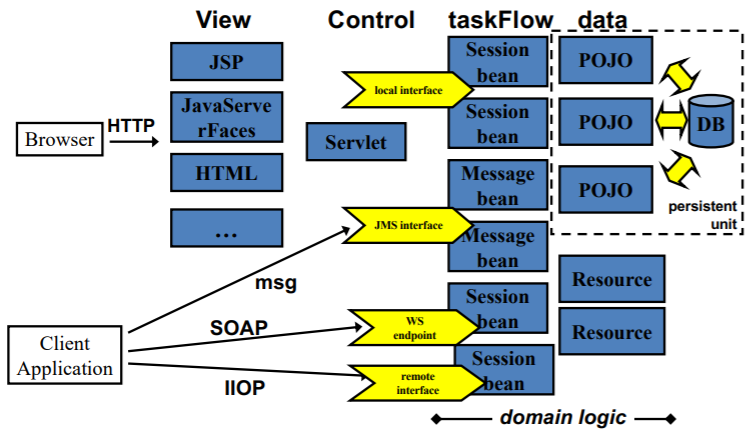
\includegraphics[scale=0.5]{Imm/j2ee-scheme.png}
\end{figure}
    
EJB è conosciuto anche come la tecnologia dei \textit{Tre Beans}: infatti oltre a Session Bean e Message Bean, i POJO (le entità persistenti) nel dominio di EJB vengono chiamati \textbf{Entity Bean}.\\

\textbf{Session Bean} è una classe che implementa interfacce locali \mintinline{Java}{@javax.ejb.Local} (i metodi possono essere invocati solo localmente), interfacce remote \mintinline{Java}{@javax.ejb.Remote} (i metodi possono essere invocati remotamente con RMI) o interfacce endpoint  \mintinline{Java}{@javax.jws.WebService} (i metodi possono essere invocati remotamente usando SOAP con JAX-RPC).\\

I \textit{Session Bean} possono essere \textbf{stateless} \mintinline{Java}{@javax.ejb.Stateless}  o \textbf{stateful}  \mintinline{Java}{@javax.ejb.Stateful}, in base a se contiene al suo interno informazioni di stato o meno. \\

\textbf{Message Bean} è una classe che implementa un’interfaccia che viene eseguita quando viene ricevuto un messaggio asincrono.
I messaggi JMS usano l’interfaccia \mintinline{Java}{javax.jms.MessageListener} e un Message Bean è marcato dall’annotazione \mintinline{Java}{@javax.ejb.MessageDriven}.

\begin{figure}[H]
    \centering
    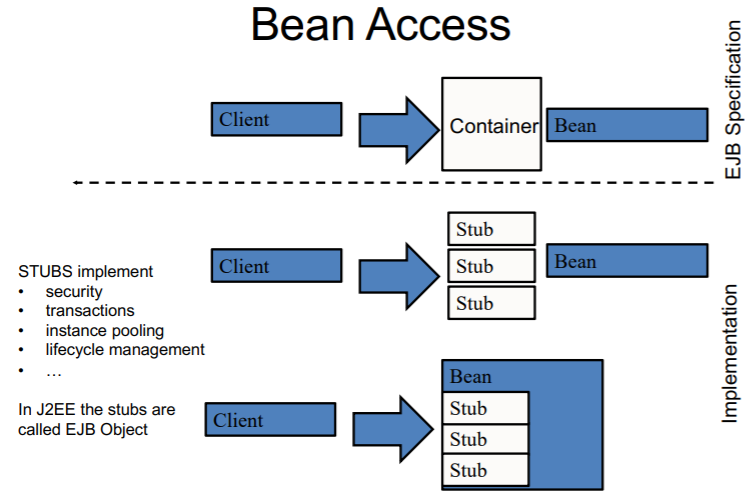
\includegraphics[scale=0.6]{Imm/bean-access.png}
\end{figure}

Le classi sono incapsulate da un elemento detto \textbf{container}, che si sovrappone tra il bean e il resto e che intercetta tutte le richieste che vengono fatte al bean.\\
Questo comportamento può essere ottenuto in diversi modi, per esempio creando componenti detti \textbf{stub} che sono indipendenti dal bean oppure instrumentando il codice della classe implementando lo stub all’interno del bean.
Attraverso questo layer (container) è possibile aggiungere una serie di servizi (sicurezza, transazioni, gestione del ciclo di vita) in modo dichiarativo.\\

Chi implementa lo standard EJB compete sul container: oltre al servizio di default che dev’essere fornito perché fa parte dello standard e sul quale c’è una competizione in termini di performance, si possono fornire servizi ulteriori.
Per configurare il comportamento del container bisogna garantire un comportamento di default, che può essere sovrascritto dalle annotazioni all’interno dei bean (definite dallo sviluppatore), che possono essere sovrascritte dai file di configurazioni esterni (definiti dall’amministratore di sistema).

\begin{figure}[H]
    \centering
    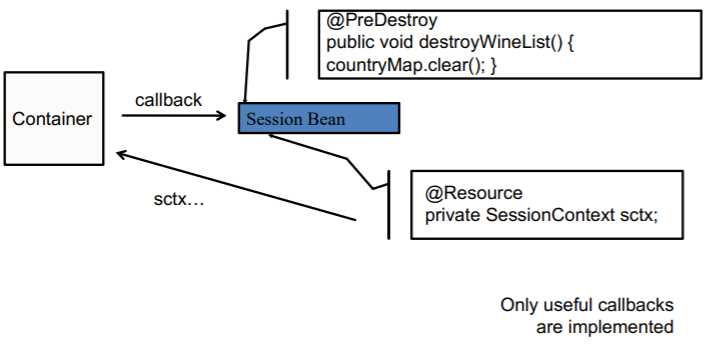
\includegraphics[scale=0.8]{Imm/session-bean.png}
\end{figure}

In alcuni casi può essere utile da un bean fare accesso al container, perché ha una serie di informazioni di contesto d’esecuzione che può essere utile recuperare.
Per farlo, si può sfruttare Dependency Injection, definendo una variabile di tipo \textbf{SessionContext} (per quanto riguarda un Session Bean) e annotarlo con  \mintinline{Java}{@Resource} per far sì che questo campo venga valorizzato con un riferimento al Container.\\

I bean hanno un ciclo di vita (creati quando serve e poi distrutti). Ciascun bean può invocare una serie di metodi invocati dal Container producendo delle \textbf{call back}, quando dei particolari eventi sono prodotti (alla creazione del bean o prima della distruzione del bean per liberare risorse).\\
Se si ha bisogno di implementare della logica che dev’essere eseguita come reazione a quegli eventi si possono usare delle annotazioni specifiche per i metodi (esempio:  \mintinline{Java}{@PreDestroy}).\\

EJB supporta sia la Dependency Injection sia il Java Naming and Directory Service (JNDS) che è un servizio di Service Locator che può essere utilizzato all’interno delle applicazioni.\\
Servizi che il container può dare a un’applicazione EJB:
\begin{itemize}
    \item \textbf{Resource Managment}: gestione efficiente delle risorse.
    \item \textbf{Services} : servizi che possono essere usati e configurati all’interno dell’applicazione.
\end{itemize}

\subsection{Resource Management}
\textbf{Instance pooling}: l’idea è quella ridurre il numero di oggetti utilizzati per servire le richieste sfruttando il Container per ottimizzare il riuso degli oggetti (in modo tale che non sia necessario creare nuovi oggetti/istanze/session bean per ogni richiesta del client). Un client non interagisce mai direttamente con il bean, in quanto le richieste vengono sempre intercettate dal container.\\

In base all’annotazione aggiunta all’interno dei Session Bean (stateless o stateful) impatta il suo utilizzo: se è stateless, può essere riutilizzato per servire richieste differenti.\\

All’inizio il bean viene creato senza uno stato e posto nel pool; quando arriva una richiesta viene pescato un bean qualsiasi nel pool che viene posto a uno stato ready per processare la richiesta e poi viene rimesso nel pool.
\begin{figure}[H]
    \centering
    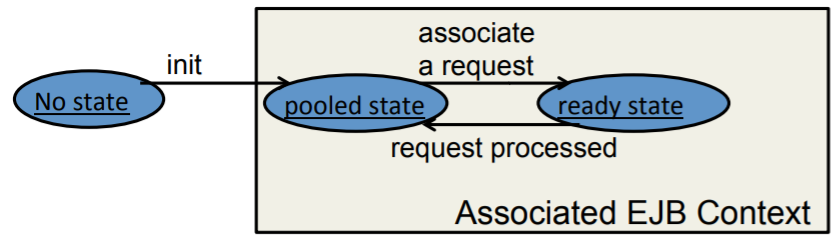
\includegraphics[scale=0.3]{Imm/res-mange_1.png}
\end{figure}

% \begin{figure}[H]
%     \centering
%     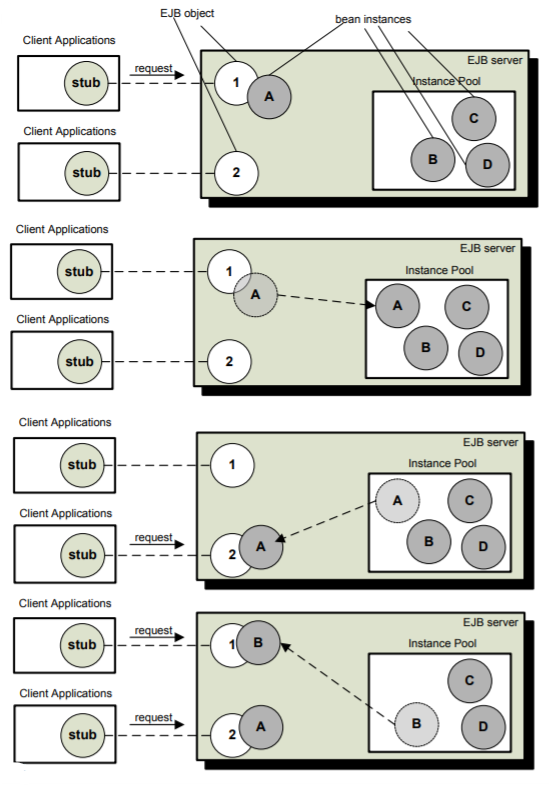
\includegraphics[scale=0.5]{Imm/res-mange_2.png}
% \end{figure}

Nel caso di bean stateful, questi possiedono uno stato e quindi non possono essere utilizzati per rispondere a richieste di client differenti. Per ottimizzare l’utilizzo della memoria, si sfrutta un meccanismo di \textbf{attivazione/passivazione}, cioè essendoci sempre l’EJB object come unico elemento di frontiera che riceve le richieste, non è necessario mantenere in memoria i bean, soprattutto se non vengono utilizzati.\\

Se un bean stateful non viene utilizzato per lungo tempo (dove lungo tempo viene definito all’interno della configurazione del framework), può essere passivizzato, quindi rimosso dalla memoria e salvato su disco, e nel momento in cui dovesse arrivare una richiesta il container (l’EJB object) può recuperare il bean, riportarlo in memoria e utilizzarlo per rispondere alla richiesta.
\subsection{Services}
Lo standard EJB specifica 8 servizi: concurrency, transaction management, persistency (JPA), distribution, naming (JNDI + Dependency Injection), security, asynchronous communication (JMS) e timer (simple generator of events). Andiamo ora a vedere alcuni dei servizi più nel dettaglio.

\subsubsection{Concorrenza}
La sua gestione sta nel fatto che non c’è concorrenza: non possono essere creati nuovi thread nei bean (non c’è concorrenza all’interno di un singolo bean).\\

C’è però concorrenza tra client multipli: ogni client ha una propria istanza (Session Bean) e quindi una propria visione dello stato di applicazione, pertanto tutti i vari bean sono concorrenti tra loro. Per quanto riguarda gli Entity Bean invece ce n’è uno per transazione, quindi non ci sono problemi di concorrenza all’interno dell’applicazione ma ci sono problemi di sincronizzazione con il DB. Gli eventuali conflitti sono gestiti con le strategie ottimistiche e pessimistiche di locking.\\

I Message Bean processano un messaggio alla volta e pertanto non generano problemi di concorrenza.


\subsubsection{Distribuzione}
Ci sono numerosi protocolli (Web, RMI, SOAP, JMS) che fanno parte dello standard che possono essere utilizzati in modo molto trasparente per far comunicare i componenti tra loro attraverso le annotazioni. Entity Bean serializzati possono essere trasferiti al client.\\
RMI è inoltre utilizzato per comunicare tra componenti EJB lato server.


\subsubsection{Sicurezza}
EJB nativamente supporta tre livelli di sicurezza: 
\begin{itemize}
    \item \textbf{authentication}: per convalidare l’identità di un utente. Comprende tecniche di autenticazione multipla.
    \item \textbf{authorization} o accesses control: applica la security policy per verificare se un utente con determinati privilegi può eseguire l’operazione richiesta. Controllo al livello di dati, sottosistemi o oggetti.
    \item \textbf{secure communications}: crea canali sicuri
\end{itemize}
La sicurezza si basa su JAAS (Java Authentication and Authorization Service).

\subsection{Transazioni dichiarative}
In EJB 3.0 le transazioni possono essere definite dichiarativamente.
\subsubsection{Annotazioni}
Le annotazioni specificano la semantica transazionale: una transazione inizia (termina) quando l’esecuzione di un metodo associato a una transazione inizia (termina). La logica di business è separata dalla logica transazionale. È possibile gestire esplicitamente le transazioni: le logiche di business e di transazione non sono più separate.\\

L’annotazione \mintinline{Java}{@TransactionAttribute} può essere usato per specificare la semantica transazionale di un metodo e può avere diverse opzioni: 
\begin{itemize}
    \item \textbf{NotSupported}: a prescindere dal contesto transazionale del chiamante, quando l’operazione viene eseguita dal bean, non viene eseguita nel contesto transazionale.
    \item \textbf{Supports}: il bean segue il contesto transazionale del chiamante (se ha aperto una transazione, l’operazione viene eseguita nel contesto transazionale e viceversa).
    \item \textbf{Required} (opzione di default): se il chiamante ha aperto una transazione, l’operazione del bean fa parte della medesima transazione; se il chiamante non ha aperto una transazione, ne viene aperta una per l’operazione del bean che si chiuderà al termine di tale operazione.
    \item \textbf{RequiresNew}: a prescindere dal contesto transazionale del chiamante, quando l’operazione viene eseguita dal bean, viene eseguita nel contesto transazionale.
    \item \textbf{Mandatory}: è responsabilità del chiamante aver creato una transazione (e viene così eseguita l’operazione nel contesto transazionale), altrimenti si ha un contesto di errore.
    \item \textbf{Never}: l’operazione non deve essere eseguita in un contesto transazionale; quindi se il chiamante ha aperto una transazione si ha un contesto di errore.
\end{itemize}

Tutte queste operazioni si applicano per i Session Bean stateless e stateful. Nel caso degli entity Bean, essendo oggetti sincronizzati con il database, le operazioni devono sempre avvenire nel contesto transazionale e quindi tipicamente vengono utilizzati Required, RequiresNew e Mandatory.\\

Per i Message Bean, che sono eseguiti in modo asincrono, le opzioni possibili sono \textbf{NotSupported} o \textbf{RequiresNew}.

\subsection{Isolation e Database Locking}
Isolamento (imperfetto), perché ha tre possibili problemi:
\begin{itemize}
    \item \textbf{Dirty Reads}: una transazione legge dati modificati da una transazione per la quale non è stato effettuato un commit.
    \item \textbf{Unrepeatable Reads}: indica che le stesse operazioni di read eseguite all’interno di una stessa transazione possono ritornare risultati differenti.
    \item \textbf{Phantom Reads}: le transazioni possono leggere nuovi record generati dopo che è iniziata la transazione (da un’altra transazione che si conclude prima).\\
    Non si tratta più della modifica ma dell’aggiunta di un record.
\end{itemize}
L’isolation perfetta è quella che introduce il costo maggiore in termini di prestazioni.\\

\textbf{Livelli di isolamento}
\begin{itemize}
    \item \textbf{Read uncommitted}: sono possibili nonrepeatable reads, dirty reads e phantom reads.
    \item \textbf{Read committed}: sono possibili nonrepeatable reads e phantom reads.
    \item \textbf{Repeatable read}: sono possibili solo i phantom reads.
    \item \textbf{Serializable}: isolamento perfetto.
\end{itemize}
Un alto livello di isolamento garantisce maggior correttezza ma basse prestazioni e viceversa, un basso livello di isolamento determina una minor correttezza ma alte prestazioni.\\

Il locking ottimistico è in alternativa al Locking resources (locking pessimistico) e richiede un campo “Versione” extra per le Entità. Il version field viene incrementato ogni volta che l’Entità viene modificata e viene controllato al momento del commit: se il version number è cambiato, viene rilevato un conflitto e si fa rollback.\\

Questa soluzione è altamente efficace quando la probabilità di rollback è bassa, altrimenti risulta essere inefficiente.
L’optimistic locking è supportato in EBJ 3.0, tramite l’annotazione \mintinline{Java}{@Version}.
\end{document}